\documentclass[10pt,a4paper]{article}

\usepackage[margin=1in]{geometry}
\usepackage[UKenglish]{babel}
\usepackage{enumitem}
\usepackage{calc}
\usepackage{fancyhdr}
\usepackage{graphicx}
\usepackage{multirow}
\usepackage[table]{xcolor}
\usepackage{float}
\usepackage{longtable}
\usepackage{tabularx}
\usepackage{parskip}
\usepackage{soul}
\usepackage{ifthen}
\usepackage[compact]{titlesec}
\usepackage[justification=centering]{caption}
\usepackage{subcaption}
\usepackage{listings}
\usepackage{xcolor}

\colorlet{punct}{red!60!black}
\definecolor{background}{HTML}{EEEEEE}
\definecolor{delim}{RGB}{20,105,176}
\definecolor{key}{RGB}{73,109,112}
\colorlet{numb}{magenta!60!black}

\lstdefinelanguage{json}{
    basicstyle=\normalfont\ttfamily,
    numbers=left,
    numberstyle=\scriptsize,
    stepnumber=1,
    numbersep=8pt,
    showstringspaces=false,
    breaklines=true,
    frame=lines,
    backgroundcolor=\color{background},
    literate=
     *{0}{{{\color{numb}0}}}{1}
      {1}{{{\color{numb}1}}}{1}
      {2}{{{\color{numb}2}}}{1}
      {3}{{{\color{numb}3}}}{1}
      {4}{{{\color{numb}4}}}{1}
      {5}{{{\color{numb}5}}}{1}
      {6}{{{\color{numb}6}}}{1}
      {7}{{{\color{numb}7}}}{1}
      {8}{{{\color{numb}8}}}{1}
      {9}{{{\color{numb}9}}}{1}
      {:}{{{\color{punct}{:}}}}{1}
      {,}{{{\color{punct}{,}}}}{1}
      {\{}{{{\color{delim}{\{}}}}{1}
      {\}}{{{\color{delim}{\}}}}}{1}
      {[}{{{\color{delim}{[}}}}{1}
      {]}{{{\color{delim}{]}}}}{1},
}
\lstset{emph={%  
    Systems, SystemID, Sensors, SensorID, Params, Engines, DatastoreGateway, Reporting
    },emphstyle={\color{key}\bfseries}%
}

\definecolor{reqColor}{RGB}{80,80,120}

%%Tables
\newcommand{\tableformat}[4]{
\begin{table}[ht!]
\centering
  \rowcolors{2}{gray!10} {white}
\def\arraystretch{1.5}
\begin{tabularx}{\textwidth}{#1}
  \hline
  \rowcolor[gray]{0.9} #2
  \hline
\end{tabularx}
\caption{#3}
\label{#4}
\end{table}}

\pagestyle{fancy}
\lhead{T Davies, A Fahie, A Fairbairn, A Free, J Mansfield, R Tucker, M 
Walker}
\chead{}
\rhead{GPIG-C}
\cfoot{\vspace{-0.6cm} \thepage}

\setlist{nolistsep} % Reduces lots of white space around lists

\renewcommand{\headrulewidth}{0.4pt} % Add rules below header
\renewcommand*{\thefootnote}{\fnsymbol{footnote}}

\newcommand{\conreq}[1]{\textcolor{reqColor}{\textbf{CR.#1}}}
\newcommand{\fr}[1]{\textcolor{reqColor}{\textbf{FR.#1}}}
\newcommand{\ed}[1]{\textcolor{reqColor}{\textbf{ED.#1}}}
\newcommand{\nfr}[1]{\textcolor{reqColor}{\textbf{NFR.#1}}}
\newcommand{\qas}[1]{\textcolor{reqColor}{\textbf{QAS.#1}}}

%%Scenarios
\newenvironment{scenario}[1]{
\newcommand{\source}[1]{\item[Source of Stimulus:] ##1}
\newcommand{\stimulus}[1]{\item[Stimulus:] ##1}
\newcommand{\artifact}[1]{\item[Artifact:] ##1}
\newcommand{\environment}[1]{\item[Environment:] ##1}
\newcommand{\response}[1]{\item[Response:] ##1}
\newcommand{\measure}[1]{\item[Response Measure:] ##1}
\newcommand{\rationale}[1]{\item[Scenario Rationale:] ##1}
\newcommand{\quality}[1]{\item[Quality:] ##1}
		\begin{description} [noitemsep]	
		\item[Scenario ID:] \qas{#1}
		}{\end{description} \vspace*{0.3cm}
		}

%%Requirements
\newenvironment{requirements}{
\newcommand{\requirement}[4]{\item[##1{##2}] ##3
							\ifx&##4&
							%nothing
							\else
								\begin{description}
									##4
								\end{description}							
							\fi
							}
		\begin{description}[noitemsep, leftmargin=1.3cm]	
		}{\end{description} \vspace*{0.3cm}
		}
		
\begin{document}
\begin{center}
{\vspace*{-0.5cm}
\Huge GPIG-C Final Report}
\vspace*{0.2cm}

Word count: @WORD_COUNT@
 (\textit{using TeXCount})
\vspace*{0.1cm}

Wednesday, 21st May 2014
\end{center}
\vspace*{0.4cm}
\hrule
\vspace*{0.4cm}

%-------------------------------------------------------------%
%----------------------INTRODUCTION -------------------%
%-------------------------------------------------------------%
\section{Introduction}
\label{sec:intro}

This report details the design and development of a Health and Usage Monitoring System (HUMS), focussing particularly on progress since the Interim Report. This includes the development of a prototype implementation that will be demonstrated to the Customer.

In Section~\ref{sec:requirements}, previously identified requirements are refined, building on Customer feedback, and a set of external dependencies are identified. The associated risks of the project are considered and risk reduction strategies are discussed in Section~\ref{sec:risks}. The quality attributes that the System must exhibit are described in Section~\ref{sec:qualities} and scenarios that require those qualities are given in Section~\ref{sec:scenarios}. To support these quality attributes, tactics and architectural design patterns are identified in Section~\ref{sec:tactics}. In Section~\ref{sec:architecture}, the design of the HUMS architecture is presented from a variety of software engineering views. The development of the prototype HUMS, which demonstrates many important features of the System, is then described in Section~\ref{sec:dev}, followed by test results in Section~\ref{sec:testing} and an evaluation of the achieved quality and functionality of the System in Section~\ref{sec:prototype}. An overview of communication with the Customer is given in Section~\ref{sec:customer_comms}. The project is then concluded in Section~\ref{sec:conclusion}, and the team reflects on their decisions throughout the project.

%-------------------------------------------------------------%
%--------------------------GLOSSARY ---------------------%
%-------------------------------------------------------------%
\section{Glossary}
\label{sec:glossary}
\begin{description}%[leftmargin=!,labelwidth=\widthof{\bfseries Data output clientxx},noitemsep]
	\item[The HUMS/System] The Health and Usage Monitoring System being developed.
	
	\vspace{0.15cm}
	\item[Customer] Thales, the organisation that has commissioned the System.
	\item[Consumer] An organisation, or individual within that organisation, using the HUMS.
	\item[Client] Consumer hardware or software that interfaces with the HUMS.
	
	\vspace{0.15cm}
	\item[Event] A trend in data identified by analysis.
	\item[Notification] A message dispatched by the System when an Event is fired.
	\item[Report] An artifact consisting of information produced by the HUMS at the request of the Consumer.
	
	\vspace{0.15cm}
	\item[Input Interface] An interface through which data is supplied to the HUMS.
	\item[Data Emitter] Software that provides data to a HUMS instance through an Input Interface.
	\item[Output Interface] An interface through which Reports and Notifications are dispatched.
	\item[Data Output Client] A Client that receives data from an Instance through an Output Interface.
    \item[Datastore] A component of the System which stores data received through an Input Interface.
    \item[(HUMS) Core] The component of the System which performs analysis and receives data from Data Emitters through Input Interfaces.
	\item[Admin Centre] A web interface to configure and interact with the HUMS Core.

	\vspace{0.15cm}
	\item[Sensor] A source of data to be monitored by the System.
	\item[Sensor ID] A unique identifier denoting a particular Sensor.
	\item[System ID] A unique identifier denoting a group of Sensors.
\end{description}

%-------------------------------------------------------------%
%-------------------REQUIREMENTS----------------------%
%-------------------------------------------------------------%
\section{Requirements Refinement}
\label{sec:requirements}
Based on Customer feedback from the previous reports, the requirements of the HUMS have been updated. This included refining existing requirements and adding newly identified requirements. The constraint requirements have been removed as they were deemed unnecessary by the module leader and, instead, the external dependencies of the system have been identified.

\subsection{Functional Requirements}
\label{sec:functional_requirements}

\emph{FR.4.1} has been refined by specifying exactly how configuration files will be used within our implementation to increase configurability. We chose to use JavaScript Object Notation (JSON) \cite{json} as the configuration format because it is lightweight and widely-used format supported by many languages and tools.

\emph{FR.12} became apparent after considering the ability to reload the configuration from \emph{FR.4.1.2}. Without the ability to dynamically load new engines, adding or removing analysis, storage and reporting engines would require a restart of the System.

\begin{requirements}
\requirement{\fr}{1}{Data Emitters shall be able to push correctly structured data to the HUMS.}{
	\requirement{\fr}{1.1}{The HUMS shall provide an API for data input (the Input Interface).}{
		\requirement{\fr}{1.1.1}{The Input Interface shall require a System ID that uniquely identifies Clients.}{}
		\requirement{\fr}{1.1.2}{The Input Interface shall require input data to be timestamped.}{}
		\requirement{\fr}{1.1.3}{The Input Interface shall allow Data Emitters to send Sensor IDs and their values to the HUMS, to be made available to an analysis engine.}{}
	}
	\requirement{\fr}{1.2}{Data Emitters for extracting data from the given test applications shall be provided.}{}
}
\requirement{\fr}{2}{The HUMS shall allocate timestamps to new data.}{
	\requirement{\fr}{2.1}{Data shall be timestamped before it reaches the Input Interface.}{}
	\requirement{\fr}{2.2}{Timestamps shall be stored alongside the input data.}{}
}
\requirement{\fr}{3}{The HUMS shall store correctly structured data.}{
	\requirement{\fr}{3.1}{The HUMS shall use a database abstraction layer, allowing the Consumer to select their choice of Datastore technology.}{}
}
\requirement{\fr}{4}{The HUMS shall store Consumer configuration files using JSON.}{
	\requirement{\fr}{4.1}{The HUMS shall allow authorised individuals to modify configuration files.}{
      \requirement{\fr}{4.1.1}{The Admin Centre shall provide an interface to allow authorised individuals to modify the configuration.}{}
      \requirement{\fr}{4.1.2}{The HUMS shall monitor the configuration for changes and apply them.}{}
    }
	\requirement{\fr}{4.2}{The configuration file shall allow the Consumer to define a storage limit.}{}
	\requirement{\fr}{4.3}{The configuration file shall allow the Consumer to set an expiry time on stored data.}{}
	\requirement{\fr}{4.4}{The configuration file shall allow the Consumer to define that, upon reaching their defined data storage quota, new data is no longer stored.}{}
	\requirement{\fr}{4.5}{The configuration file shall allow the Consumer to define that, upon reaching their defined data storage limit, old data is removed to make room for the new data.}{}
}
\requirement{\fr}{5}{The HUMS shall dispatch a Notification when the Consumer's storage limit is reached.}{}
\requirement{\fr}{6}{The HUMS shall store no more data records than the Consumer-defined storage quota.}{}
\requirement{\fr}{7}{Events shall be triggered in response to data matching analysis rules specified by the Consumer.}{
	\requirement{\fr}{7.1}{The HUMS shall allow the Consumer to specify which analysis rules will produce Events.}{}
	\requirement{\fr}{7.2}{The HUMS shall allow the Consumer to define their own Events.}{}
	\requirement{\fr}{7.3}{The HUMS shall provide an API, allowing analysis engines to fetch stored data.}{}
	\requirement{\fr}{7.4}{Events shall be identified by analysis engines.}{}
	\requirement{\fr}{7.5}{The HUMS shall provide a simple analysis engine in the form of a rules engine.}{}
}
\requirement{\fr}{8}{After dispatching a Notification for an Event of a particular type, no more Notifications for an Event of that type shall be sent during a Consumer-specified cool down period.}{
	\requirement{\fr}{8.1}{The HUMS shall allow the Consumer to specify a cool down period for particular Events.}{}
}
\requirement{\fr}{9}{The HUMS shall generate Notifications in response to Events using the registered Notification Engines.}{}
\requirement{\fr}{10}{The HUMS shall interface with Report engines, allowing them to pull Reports.}{}
\requirement{\fr}{11}{The System shall allow for Notifications to be fed back to Client to change the way in which data is sensed.}{}
\requirement{\fr}{12}{The System shall load new engines added by an authorised user at both runtime and compile time.}{}
\end{requirements}

\subsection{Non-Functional Requirements}
\label{sec:nonfunctional_requirements}

\emph{NFR.14} has been added as a Consumer will not necessarily want to use the Admin Centre to modify the system configuration, in which case it should be possible to manually amend the configuration file.

\begin{requirements}
\requirement{\nfr}{1}{The HUMS shall undergo hardware modifications without loss of previously stored data.}{}
\requirement{\nfr}{2}{Consumers shall be provided with documentation detailing how to use the HUMS.}{}
\requirement{\nfr}{3}{The HUMS shall be accessible to Consumers regardless of their geographic location.}{}
\requirement{\nfr}{4}{The HUMS shall only accept data from a Client of the Input Interface providing valid credentials.}{}
\requirement{\nfr}{5}{The HUMS shall allow data to be stored according to the relevant industry security standards.}{}
\requirement{\nfr}{6}{The HUMS shall be tested to ensure all requirements are met before deployment.}{
	\requirement{\nfr}{6.1}{The HUMS shall be tested using unit testing.}{}
	\requirement{\nfr}{6.2}{The HUMS shall be tested using integration testing.}{}
	\requirement{\nfr}{6.3}{The HUMS shall be tested using system testing.}{}
	\requirement{\nfr}{6.4}{The HUMS shall be tested using inspection.}{}
	\requirement{\nfr}{6.5}{The HUMS shall be tested using acceptance testing.}{}
}
\requirement{\nfr}{7}{The Customer shall complete acceptance testing before the System is deployed.}{}
\requirement{\nfr}{8}{The System shall be able to support at least five Clients of the Output Interface per HUMS instance.}{}
\requirement{\nfr}{9}{The System shall be available for no less than 99.9\% of each month.}{}
\requirement{\nfr}{10}{Data shall be backed up within 24 hours of having been made available to the System.}{}
\requirement{\nfr}{11}{Timestamps applied by the system shall be accurate to within 5~ms of UTC.}{}
\requirement{\nfr}{12}{The System shall dispatch Notifications within 5~ms of an Event being triggered.}{}
\requirement{\nfr}{13}{The System shall support storing data without requiring specific schemata.}{}
\requirement{\nfr}{14}{The configuration file shall be in a human-readable format.}{}
\end{requirements}

\subsection{External Dependencies}
\label{sec:external_dependencies}

External dependencies are requirements outside the scope of development that are necessary for the HUMS to be deployed successfully. The previous report did not consider external dependencies pertaining to the Consumer running the HUMS, as well as those of the development process, so they are considered here.

 \begin{description}
 \item[\ed{1}] The provisioned deployment platform must be running an up-to-date Java Virtual Machine (JVM) in a GNU/Linux, Windows or OS X environment.
 \item[\ed{2}] Any necessary network or firewall configuration must be performed to allow Clients to communicate with the Core where necessary.
  \item[\ed{3}] The selected remote data stores must have a high enough availability to meet the non-functional requirements of the HUMS set out earlier.
 \end{description}
% \item[\ed{3}] The HUMS and Customer test applications must be compatible, allowing the HUMS to sensor, storage, analyse and notify regarding the test applications in such a way that no data is lost. % Doesn't sound like an External Dependancy to me?

%-------------------------------------------------------------%
%--------------------------RISKS--------------------------%
%-------------------------------------------------------------%
\section{Project Risks}
\label{sec:risks}
It is important to consider the risks of any software project so that appropriate mitigation strategies can be applied and clear contingency plans can be put in place to prevent any potential problems having a large impact. This will help to ensure that all work is completed within project constraints and to a high standard. For this phase of the project, risks have been identified and contingencies put in place before beginning development, unlike in previous phases during which risks were mitigated as the occurred.

Unlike in the previous reports, risks have been separated into personnel risks and technical risks. This distinction was not made previously and resulted in technical risks being sidelined and inadequately considered. Personnel risks are presented in Table~\ref{tab:human_risks} and technical risks in Table~\ref{tab:tech_risks}. Some risks from the Interim Report have been modified, while others are new and specific to the revised system architecture. Each risk has been assigned a risk level corresponding to the product of their likelihood and impact, as described by \cite{risks}, where likelihood is a value in the range 1--100 where 100 is a high likelihood.

\tableformat{ p{0.8cm} X X X c c c }
{ 	\hline
  	Risk ID & Risk \newline Description & Impact \newline Description & Contingency & Prob. (\%) & Impact & Score \\
  	\hline
  
    R.1 & Loss of team member(s) or team member(s) underperform. & Internal/external deadline failure. Poor standard of work. & Reallocate work across remaining team members and notify module leader. & 10 & Moderate & \textbf{Low} \\
    R.2 & External pressures (such as other modules) limit the amount of development time. & Internal/external deadline failure. Lack of technical achievement. & Modify the project plan to reduce the prototype functionality. Request extension. & 25 & Moderate &  \textbf{Low} \\
    R.3 & Customer does not think that the HUMS design correctly fulfils their brief. & Wasted time. Failure to meet deadlines. Limited prototype implementation. & Modify the system and communicate with the customer to ensure the HUMS design is as they expect. & 15 & Serious &  \textbf{Low} \\
    R.4 & Work is lost due to human or hardware error. & Wasted time. Failure to meet deadlines. Limited prototype implementation. & Revert to a backup and continue working from there, possibly reducing system functionality. & 30 & Minor &  \textbf{Low} \\
    R.5 & The Consumer fails to update the configuration files of the HUMS. & Consumers find the system difficult to use and decide to use a different, simpler HUMS. & Survey potential Consumers to discover what they would find simplest to use and then implement such a system. & 20 & Medium & \textbf{Low} \\	
}
{The human and business risks associated with this phase of the project.}{tab:human_risks}


\tableformat{ p{0.8cm} X X X c c c }
{ 	\hline
    Risk ID & Risk \newline Description & Impact \newline Description & Contingency & Prob. (\%) & Impact & Score \\
  	\hline
  
    R.6 & Developed Admin Centre does not satisfy the outlined requirements. & Poor user experience. Wasted time. Failure to meet requirements. & Redesign Admin Centre. & 10 & Minor & \textbf{Low} \\
    R.7 & Data intercepted between the HUMS Core and registered engines or Datastore. & Loss of confidence in HUMS. Lost or corrupted data. & Additional penetration testing to identify security flaws. Have an audit trail. & 5 & Serious &  \textbf{Low} \\
    R.8 & HUMS does not facilitate data storage using a variety of Datastores. & Failure to meet key modifiability, interoperability and configurability requirements. Low quality solution. & Test this system on a number of popular Datastore implementations and make any required alterations. & 20 & Serious & \textbf{Medium} \\
    R.9 & Computation by included analysis engines too slow. & Failure to meet performance targets. Loss of data due to backlog. & Re-engineer analysis system and reduce complexity. Possibly reduce the functionality of the engines. & 25 & Moderate & \textbf{Low} \\	
    R.10 & Included notification engines too slow. & Failure to meet performance targets. Loss of events, Consumer not informed of System failure. & Re-engineer notification system, reducing complexity. Possibly change protocols and functionality to meet performance requirements. & 20 & Moderate & \textbf{Low} \\	
}
{The technical risks associated with this phase of the project.}{tab:tech_risks}

\subsection{Risk Mitigation}
The following risk mitigation strategies have been applied throughout this phase of the project, during both project planning and development. In addition to the techniques specified in this section, the tactics and patterns explained in Section~\ref{sec:tactics} also help to mitigate technical risks which affect the quality of the system.

\begin{description}
\item[Scrum]
The use of the scrum as part of our software engineering methodology, as discussed in the Initial Report, helps to mitigate risks \emph{R.1--3}. The scrum allows team members to be kept up to date on what others are working on and the state of the project as a whole, making it easier for work to be reallocated between team members. It also helps to ensure decisions concerning the HUMS design are discussed and agreed upon, reducing the risk of straying away from the Customer's specification.

\item[Version Control]
The Git version control system is used, allowing the entire team to simultaneously modify the project whilst keeping a reversible history of changes. This helps to mitigate the majority of the identified risks. Personnel risks are mitigated as the team has access to the work of other members, making it easy to take over when members are unavailable, and preventing large amounts of work being lost due to human or hardware errors. Technical risks are mitigated as it is easy to identify and revert changes which may have caused a problem in the System or caused the System to not meet Customer expectations.

\item[Automated Testing] 
Automated integration, unit, and regression testing is used throughout the project, using JUnit and Mockito where necessary to ensure the HUMS implementation is stable and free of major bugs. This reduces risks \emph{R.6--10}, helping to automatically validate system requirements. Static testing is also performed using static code analysis tools in order to reduce the time spent debugging. The performance of the System is assessed with a profiler. All of these techniques help to mitigate all of the above technical risks.
\end{description}

%-------------------------------------------------------------%
%-----------------------QUALITIES-------------------------%
%-------------------------------------------------------------%
\section{Quality Attributes}
\label{sec:qualities}
Quality attributes are non-functional qualities used to measure the performance and standard of a system. They must be considered when designing the HUMS architecture to ensure that architectural decisions not only provide the desired functionality, but also result in a system meeting the quality requirements of all stakeholders.
Defining these attributes explicitly allows tactics and design patterns to be adopted at an early stage, allowing the system to achieve the desired utilities of each quality. 
Table~\ref{tab:qualities} ranks the quality attributes associated with the system and rationalises these rankings. This was not performed in the previous report, but it is important at this phase because improving one quality attribute may result in another being reduced. Achieving the right balance is very important, and the support of lower ranked qualities may need to be sacrificed in order to support the highly ranked qualities. Tailorability has been identified as particularly important to the Customer and has been decomposed into a number of sub-qualities: Modifiability, Configurability, and Interoperability.

\tableformat{ p{2.4cm} p{1.2cm} X }{
\hline
Quality \newline Attribute & Rank & Reasoning \\
\hline
Configurability & High & It is important that the HUMS can be used in a range of domains; this has been strongly emphasised by the Customer. 
\\
Modifiability & High & The HUMS will initially be built to tackle a single domain (software application), however in the future it will be used in domains such as embedded, electrical, and mechanical systems. A System which is not modifiable will be timely and costly to extend and improve. In addition, both users and developers need to be able to add custom engines to the HUMS.
\\
Interoperability & High & Interoperability is very important to the HUMS as its main purpose is to interface and exchange data with external systems.
\\
Availability & High & The non-functional system requirements identified high availability targets for the System. In addition, the HUMS is designed to be used to monitor the health of other systems, so if it is not highly available then Consumers will lose confidence in it. The HUMS must be at least as available on average as any Consumer system in order to monitor it properly.
\\
Security & High & Security is highly ranked, as data being monitored must be kept both confidential and safe. It must be impossible for an unauthorised user to view or modify System data, and data in transit between Data Emitters and the HUMS must be protected.
\\
Performance & Medium & The HUMS is required to receive data from Sensors, and produce Notification events in response to that data with a latency no greater than $5$~ms. It must also interface with many Data Emitters and Data Output Clients, meaning it must be capable of handling a large number of events quickly.
\\
Testability & Medium & The TDD development approach, discussed in the Initial Report and followed throughout the project, makes testability of medium importance to the System. Having high testability will help to reduce System faults and is also likely to increase its availability.
\\
Usability & Medium & Usability was not deemed of great importance to the System as its sub-qualities, such as learnability, have little scope to be optimised in the HUMS. Usability does need to be considered for all Consumer facing interfaces, both graphical and otherwise. Usability is likely to become more important in future development, when the focus is on deploying to real users.
\\
}{The ranked quality attributes associated with the HUMS.}{tab:qualities}


%-------------------------------------------------------------%
%----------------------SCENARIOS---------------------%
%-------------------------------------------------------------%
\section{Quality Attribute Scenarios}
\label{sec:scenarios}
Having identified key quality attributes, a set of quality attribute scenarios have been identified which show how the System should behave while supporting those quality attributes. This helps to create goals against which the final implementation can be tested to assess its quality and how effective it is at achieving its non-functional requirements. The selection of scenarios presented below are included as they highlight quality attributes and describe how the system should behave in both normal and extreme situations. Other scenarios were also considered and documented, but could not however be included due to space limitations.

\begin{scenario}{1}
\quality{Configurability}
\source{The Consumer}
\stimulus{The Consumer wishes to modify the HUMS behaviour by updating their configuration file.}
\artifact{HUMS Core, configuration file}
\environment{Runtime/compile time}
\response{The Consumer is able to modify their configuration file.}
\measure{The HUMS is not reinstalled or recompiled.}
\rationale{This scenario is important to the Customer as they expect the Consumer to be able to easily modify HUMS parameters, making it applicable to their domain, for example, by modifying the engines their Systems use. Achieving this scenario will help our solution transfer between different domains easily.}
\end{scenario}

\begin{scenario}{2}
\quality{Modifiability}
\source{Developer}
\stimulus{The Customer wishes to add an additional analysis, reporting, or notification engine to the HUMS.}
\artifact{HUMS Core}
\environment{Runtime}
\response{The new engine is implemented, tested and successfully added to the HUMS, without any loss in service.}
\measure{No other System elements are affected, and the work is completed within their budget.}
\rationale{This scenario is important to both the HUMS developers and Consumers. The HUMS should allow both of these groups to add custom engines to the System without affecting other System components.}
\end{scenario}

\begin{scenario}{3}
\quality{Security}
\source{An unknown external Client}
\stimulus{The unknown external Client attempts to access stored HUMS data or HUMS services.}
\artifact{HUMS Core}
\environment{Normal Operation -- Online}
\response{The Client is authenticated, and allowed to access System services, or is not recognised and blocked from accessing System data and services.}
\measure{No HUMS data or services are damaged as a result of the access attempt.}
\rationale{This scenario shows how the HUMS is expected to behave when a Client attempts to access its services, showing the importance of authenticating Clients and how the HUMS should respond to unauthorised Clients.}
\end{scenario}

\begin{scenario}{4}
\quality{Availability}
\source{Datastore module}
\stimulus{The Consumer's registered Datastore is unavailable to the HUMS instance.}
\artifact{HUMS}
\environment{Runtime}
\response{A Notification is sent to the administrator of the HUMS instance, and the HUMS periodically attempts to reconnect to the Datastore.}
\measure{End user defined repair time.}
\rationale{This scenario shows how the HUMS should respond to a Datastore failure, clearly drawing a line between the responsibilities of the HUMS and of the Consumer. If the Consumer's Datastore fails, the HUMS can only alert the user and attempt to reconnect; this is a critical fault and does not allow the System to be run in a degraded mode.}
\end{scenario}


%-------------------------------------------------------------%
%--------------TACTICS / PATTERNS----------------------%
%-------------------------------------------------------------%
%   Notes: 									 %
%  		- Reference risks constantly, lots and lots	 %
%-------------------------------------------------------------%

\section{Tactics and Design Patterns}
\label{sec:tactics}
Based on the key quality attributes and the identified quality attribute scenarios, the tactics and software engineering design patterns required to ensure the desired utility of these attributes can be examined. In this section we focus on those qualities ranked highly in Table~\ref{tab:qualities}.

\subsection{Tactics}

Below, the tactics that are most suitable for the HUMS are summarised. Each quality attribute has different tactics, which can be used to increase its utility within the HUMS. Configurability tactics are not included as they are covered under modifiability and interoperability and are complementary. The tactics used are based on the descriptions provided by Software Architecture in Practice~\cite{Bass98}.

\begin{description}
\item[Modifiability] \hfill
	\begin{description}[noitemsep]
	\item[Defer Binding Time] Configuration files, runtime registration and polymorphism will be used to reduce the time taken to make changes, and to allow the Consumer to modify the System at runtime.
	\item[Localise Modifications] Steps are to be taken to maintain semantic coherence within the implementation, with the team aiming to produce loosely coupled modules with high cohesion. Modules are to be generalised where possible, allowing them to preform a larger variety of functions without code changes.
	\item[Prevent Ripple Effect] Communication paths are to be restricted where possible, with the modules which can share data being limited. Information can also be hidden by using private functions, meaning changing implementation details will not affect the public APIs used by the Consumer.
	\end{description}
\item[Interoperability] \hfill
	\begin{description}[noitemsep]
		\item[Locate] Services may need to be discovered at runtime.
		\item[Managing Interfaces] Complex interactions between the HUMS Core and external engines may need to be orchestrated in order to fulfil the required functionality.
	\end{description}
\item[Availability] \hfill
	\begin{description}[noitemsep]
	\item[Fault Prevention] Bundling related actions into atomic transactions should prevent the System from entering an inconsistent state. If a single action fails within a transaction, all operations will roll back to the previous valid state. Monitoring and shutting down failed processes (e.g. failure of an analysis engine) allows for damage due to erroneous operation to be minimised.
	\item[Fault Detection] Exceptions can be used throughout the software to detect and handle errors. Ping/echo could also be used to ensure external components registered with the HUMS Core are available.
	\item[Fault Recovery] Having active or passive redundant systems would allow for automatic switchover in the event of a System failure, thus minimising any interruption that Clients experience.
	\end{description}
\item[Security] \hfill
	\begin{description}[noitemsep]
	\item[Resisting Attacks] Using prepared statements would mitigate the threat of SQL injection attacks. All connections to the Datastore will require authentication and communications should be encrypted to avoid man-in-the-middle attacks. Access to functionality should be restricted such that no individual has access to services they do not need. 
	\item[Detecting Attacks] Trap files could be used, which should only ever be accessed from specific addresses.
	\item[Recovering From Attacks] Redundant copies of data should be stored, as well as frequent data snapshots, allowing for the HUMS to roll back to a valid state after an attack.
	\end{description}
\end{description}

\subsection{Design Patterns}

A number of software design patterns have been chosen which realise the above tactics:

\begin{description}
\item[Observer] The observer pattern is a behavioural pattern that defines a one-to-many relationship between a single subject and many observers. Observers are kept in a list within the subject andare sent updates when the state of the subject changes. This will be used for the implementation of our analysis, storage, and notification engines, with controller objects keeping a list of engine observers. When the controller receives an update it can inform the relevant engines through a method call.
\item[Pipes and Filters] The adoption of the pipes and filters pattern allows for large processing tasks to be broken down into sequences of smaller independent filters, and the protocol of the data passed between those filters to be explicitly defined. Pipes and filters also increase the tailorability of the HUMS, as alternative architectures can be composed by connecting alternate filters to different pipes.
\item[Table Data Gateway] Using the table data gateway pattern, defined by \cite{fowler2002patterns} as a single object which handles all interactions with a Datastore (e.g. SQL statements), will reduce coupling and allow a single HUMS to interact with a number of different Datastores. It does so by ensuring the Core is not coupled to a particular Datastore implementation. Instead, each Datastore implements its own table data gateway which can be interchanged both at runtime and compile time. The single point of access and encapsulation means that the System as a whole is unaffected by changes to the Datastore or data access logic and therefore facilitates easier maintenance.
\item[Row Data Gateway] A row data gateway is an object which encapsulates a single record in a Datastore~\cite{fowler2002patterns}. This could be utilised by our HUMS as a method of ensuring data pulled from various Datastores can be used throughout the Core as if it had originated from a single Datastore. This will reduce the effect of impedance mismatch whilst increasing the tailorability of our solution and decreasing coupling.
\end{description}

\section{Views of the System Architecture} 
\label{sec:architecture}

Building on the architectural designs presented in the Interim Report, four more detailed views of our HUMS architecture are given in this section. We have chosen to take inspiration from the SEI~\cite{Bass98} approach to software architecture, including a \emph{Module View}, a \emph{Component and Connector View}, a dynamic \emph{Behavioural View} and finally an extensive \emph{Allocation View}.

\subsection{Module View}
\label{sec:views}
A \emph{Module View} of the HUMS, shown in Figure~\ref{fig:modules}, describes our architecture from a structural perspective in terms of a collection of components. Each component is encapsulated in order to minimise the propagation of modifications to the system.

This view is targeted at all System stakeholders, showing enough detail for developers to understand the structure and interactions between components, but not so much detail that non-technical stakeholders would be confused.

In the previous report many of the details in the module view were omitted. In this iteration details of the included and customisable components, such as the engines, are included showing exactly which modules have been implemented so far, as well as their associated interfaces which would be used by the Consumer. 

Figure~\ref{fig:modules} shows a clear separation between those modules included as part of the HUMS (in blue) and those which may be implemented by the Consumer (in green). The variety and extensiveness of our existing engine implementations already show that our System is highly tailorable, with plenty of scope for adding additional functionality.

The design patterns described above can be seen within this view, including the table data gateway pattern which is used for abstracting away the implementation details of particular Datastores, and the observer pattern implemented through the controllers and engines.

The components of the Consumer facing API, made up of generic engines and emitters, are described below:
\begin{description} [noitemsep]	
	\item[Analysis Engines] All Consumer analysis engines must extend the \texttt{AnalysisEngine} abstract class, and therefore implement the \texttt{analyse()} method. This method takes a \texttt{ClientSystem} object, which wraps information about a particular system loaded from the configuration file and returns an \texttt{Event} object generated as a result of the analysis (which may be \texttt{null}). This Event object stores the ID of the Client that generated it and key-value pairs describing the event. This gives analysis engines free reign when defining events and what information they store about those events.
	\item[Notification Engines] Notification engines must extend from the \texttt{NotificationEngine} abstract class, and therefore implement the \texttt{send()} method. The send method takes an \texttt{Event}, representing the result of analysis, and notifies the relevant individual, software, or hardware as defined. Consumers can implement this interface themselves or extend an existing implementation.
	\item[Storage Engines] Storage engines must extend from the \texttt{SystemDataGateway} abstract class, and implement four methods for interacting with a Datastore. There are two methods for writing and two for reading. The \texttt{readMostRecent()} method returns the $n$ most recent records for a given Sensor, and the \texttt{readBetween()} method returns all records for a Sensor within a time period. Both methods for reading return a \texttt{QueryResult} object, which encapsulates the values in the Datastore which fit the query. The methods for writing to a Datastore are both named \texttt{write()}, however one takes a single item of data and writes it to the Datastore and the other is a batch method, used for writing a list of data points more efficiently in the underlying implementation. 
	\item[Data Emitters] Data Emitters read values from Sensors in any format, translate them to a standard format and forward them to the Core for processing. To do this, they must implement the Input Interface. The prototype includes a number of example Data Emitters, such as the Earthquake Emitter and the Test App Emitters which are used for demonstrating the prototype. However, it is expected that Data Emitters be developed for each Consumer system. This method of data input allows data from different Clients to pass through the HUMS Core as if it was all the same, vastly increasing our solution's interoperability with different types of Client.
\end{description}

\begin{figure}[t]
  \centering
  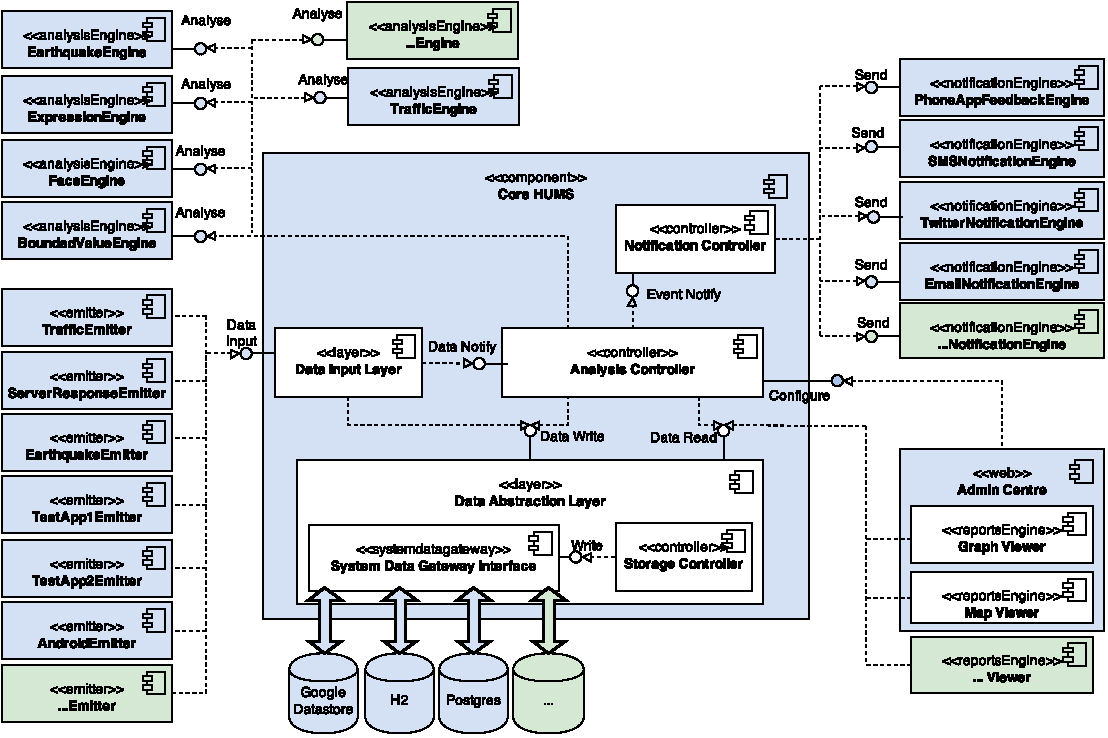
\includegraphics[width=\textwidth]{images/component.pdf}
  \caption{A \emph{Module View} of the System. Components within the blue areas are included with the HUMS. The green components are those which can be added by the Consumer to extend the HUMS to meet their needs.}
  \label{fig:modules}
\end{figure}

\subsection{Component and Connector View}
In order to visualise how data flows through the System, a \emph{Pipes and Filters} diagram of the HUMS has been created. Each filter within the diagram transforms the data received on its input pipe into the data at its output pipes. This diagram, shown in Figure~\ref{fig:pipesAndFilter}, shows the distinct data transformation and processing filters in our solution, as well as the protocol of the pipes connecting them.

Designing this diagram helped us to determine which pipes we must choose protocols for and which can be left for the client to define, improving the tailorability of the system by not unnecessarily restricting the Consumer. This view is again primarily targeted at technical stakeholders, allowing them to visualise the flow of data and determine what within the System they can configure.

The input to the HUMS, in this view, is the Sensor data from the Consumer system. This can be passed to the \texttt{:Emit Data} filter in any format, as this is the stage which converts client data to HUMS data. The \texttt{:Emit Data} filter transforms the client data into a format which can be sent using \emph{Protocol Buffers} to the \texttt{:Read Data} filter. The use of \emph{Protocol Buffers} allows for data to be sent locally or over a network, with or without encryption. 

The \texttt{:Read Data} filter deserialises the client data and transforms it to a format which can be used with the Consumer's defined Datastore. The \texttt{:Store Data} filter inserts the data into the Consumers defined Datastore.

The protocol of the pipes used to pass data to the \texttt{:Store Data} and the \texttt{:Create Report} filters are defined by the Consumer, being limited only by what their defined Datastores support. The \texttt{:Create Report} filter transforms data from the Datastore into a \texttt{Data Report}, for example, a graph or PDF document.

When sending data between the \texttt{:Store Data} and \texttt{:Analyse Data} filters, \texttt{SensorState} objects are passed, each of which hold the ID of a particular Sensor, the timestamp of when it was created and stored, and its value at the time of creation. The \texttt{:Analyse Data} filter transforms \texttt{SensorState} objects into \texttt{Event} objects, which are used by the \texttt{:Generate Notification} filter to produce Notifications using the engines specified by the Consumer.

An \texttt{Event} object contains the ID of the system that caused the event, and a \texttt{Map} of key-value pairs containing information needed by the registered notification engines. The \texttt{:Generate Notification} filter transforms an \texttt{Event} object into a Notification; for example, an SMS or email. 

\begin{figure}[ht]
  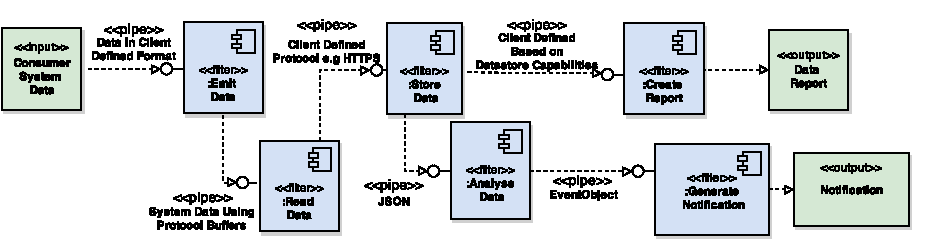
\includegraphics[width=\textwidth]{images/pipesAndFilters.pdf}
  \caption{A \emph{Component and Connector} diagram of the HUMS, showing the protocols used when passing data between filters.}
  \label{fig:pipesAndFilter}
\end{figure}

\subsection{Behavioural View}

The \emph{Behavioural View} shows the actions taken by the HUMS when data flows through the System, displaying the different components and how they interact. Figure~\ref{fig:sequence} shows a sequence diagram that presents this information, detailing the different elements of the HUMS Core and how it behaves during normal operation. Various methods and invocations are listed in the order that they occur, from top to bottom and left to right. The external Clients are omitted, as this view purely describes the HUMS Core.

\begin{figure}[h]
  \centering
  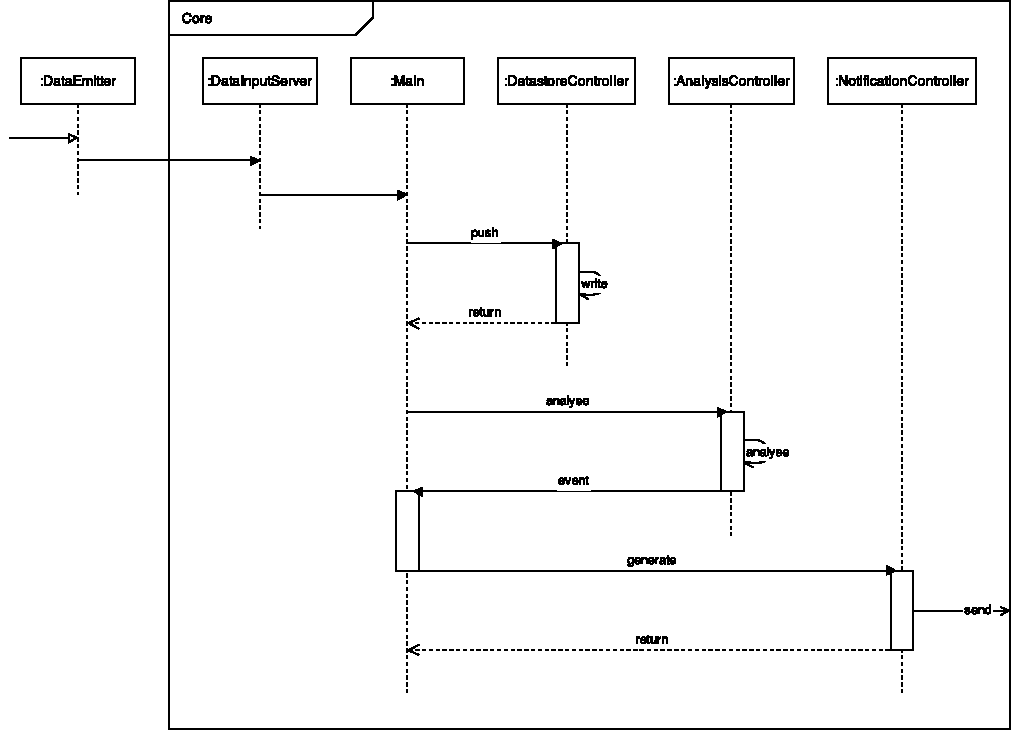
\includegraphics[width=\textwidth]{images/behaviourView.pdf}
  \caption{A sequence diagram showing the behaviour of the HUMS, using UML 2.0 notation.}
  \label{fig:sequence}
\end{figure}

\subsection{Allocation View}

The \emph{Allocation View} shows how System components may be assigned to physical hardware. It demonstrates various configurations in which the System can operate, each of which is useful in particular situations. The HUMS is designed such that, if necessary, its components can be distributed amongst a number of devices, perhaps at different geographical locations. This is achieved by allowing each component to execute in its own environment, between which data is transferred via network protocols. The deployment diagrams in Figure~\ref{fig:deployisolated} through Figure~\ref{fig:deploydemo} represent various allocations of System components. In these figures, blue components are those deployed as a service, while green components are those deployed by the Consumer.

Figures~\ref{fig:deployisolated} and~\ref{fig:deploydistributed} show configurations in which the System is entirely deployed by the Consumer. In Figure~\ref{fig:deployisolated}, the Consumer's system is deployed on an isolated device and so must also be monitored from that device. In this case, the Consumer's system emits data to the local Core, which stores that data in a local Datastore and processes it. When an Event occurs, the Core may notify the Consumer's system with feedback. In Figure~\ref{fig:deploydistributed}, the System components are distributed across a number of devices. This shows that the Consumer system may emit data to a remote HUMS Core, which may store data on a dedicated Datastore server. In this configuration, an HTTP server provides a web interface to configure the HUMS.

\begin{figure}[htp]
  \centering
  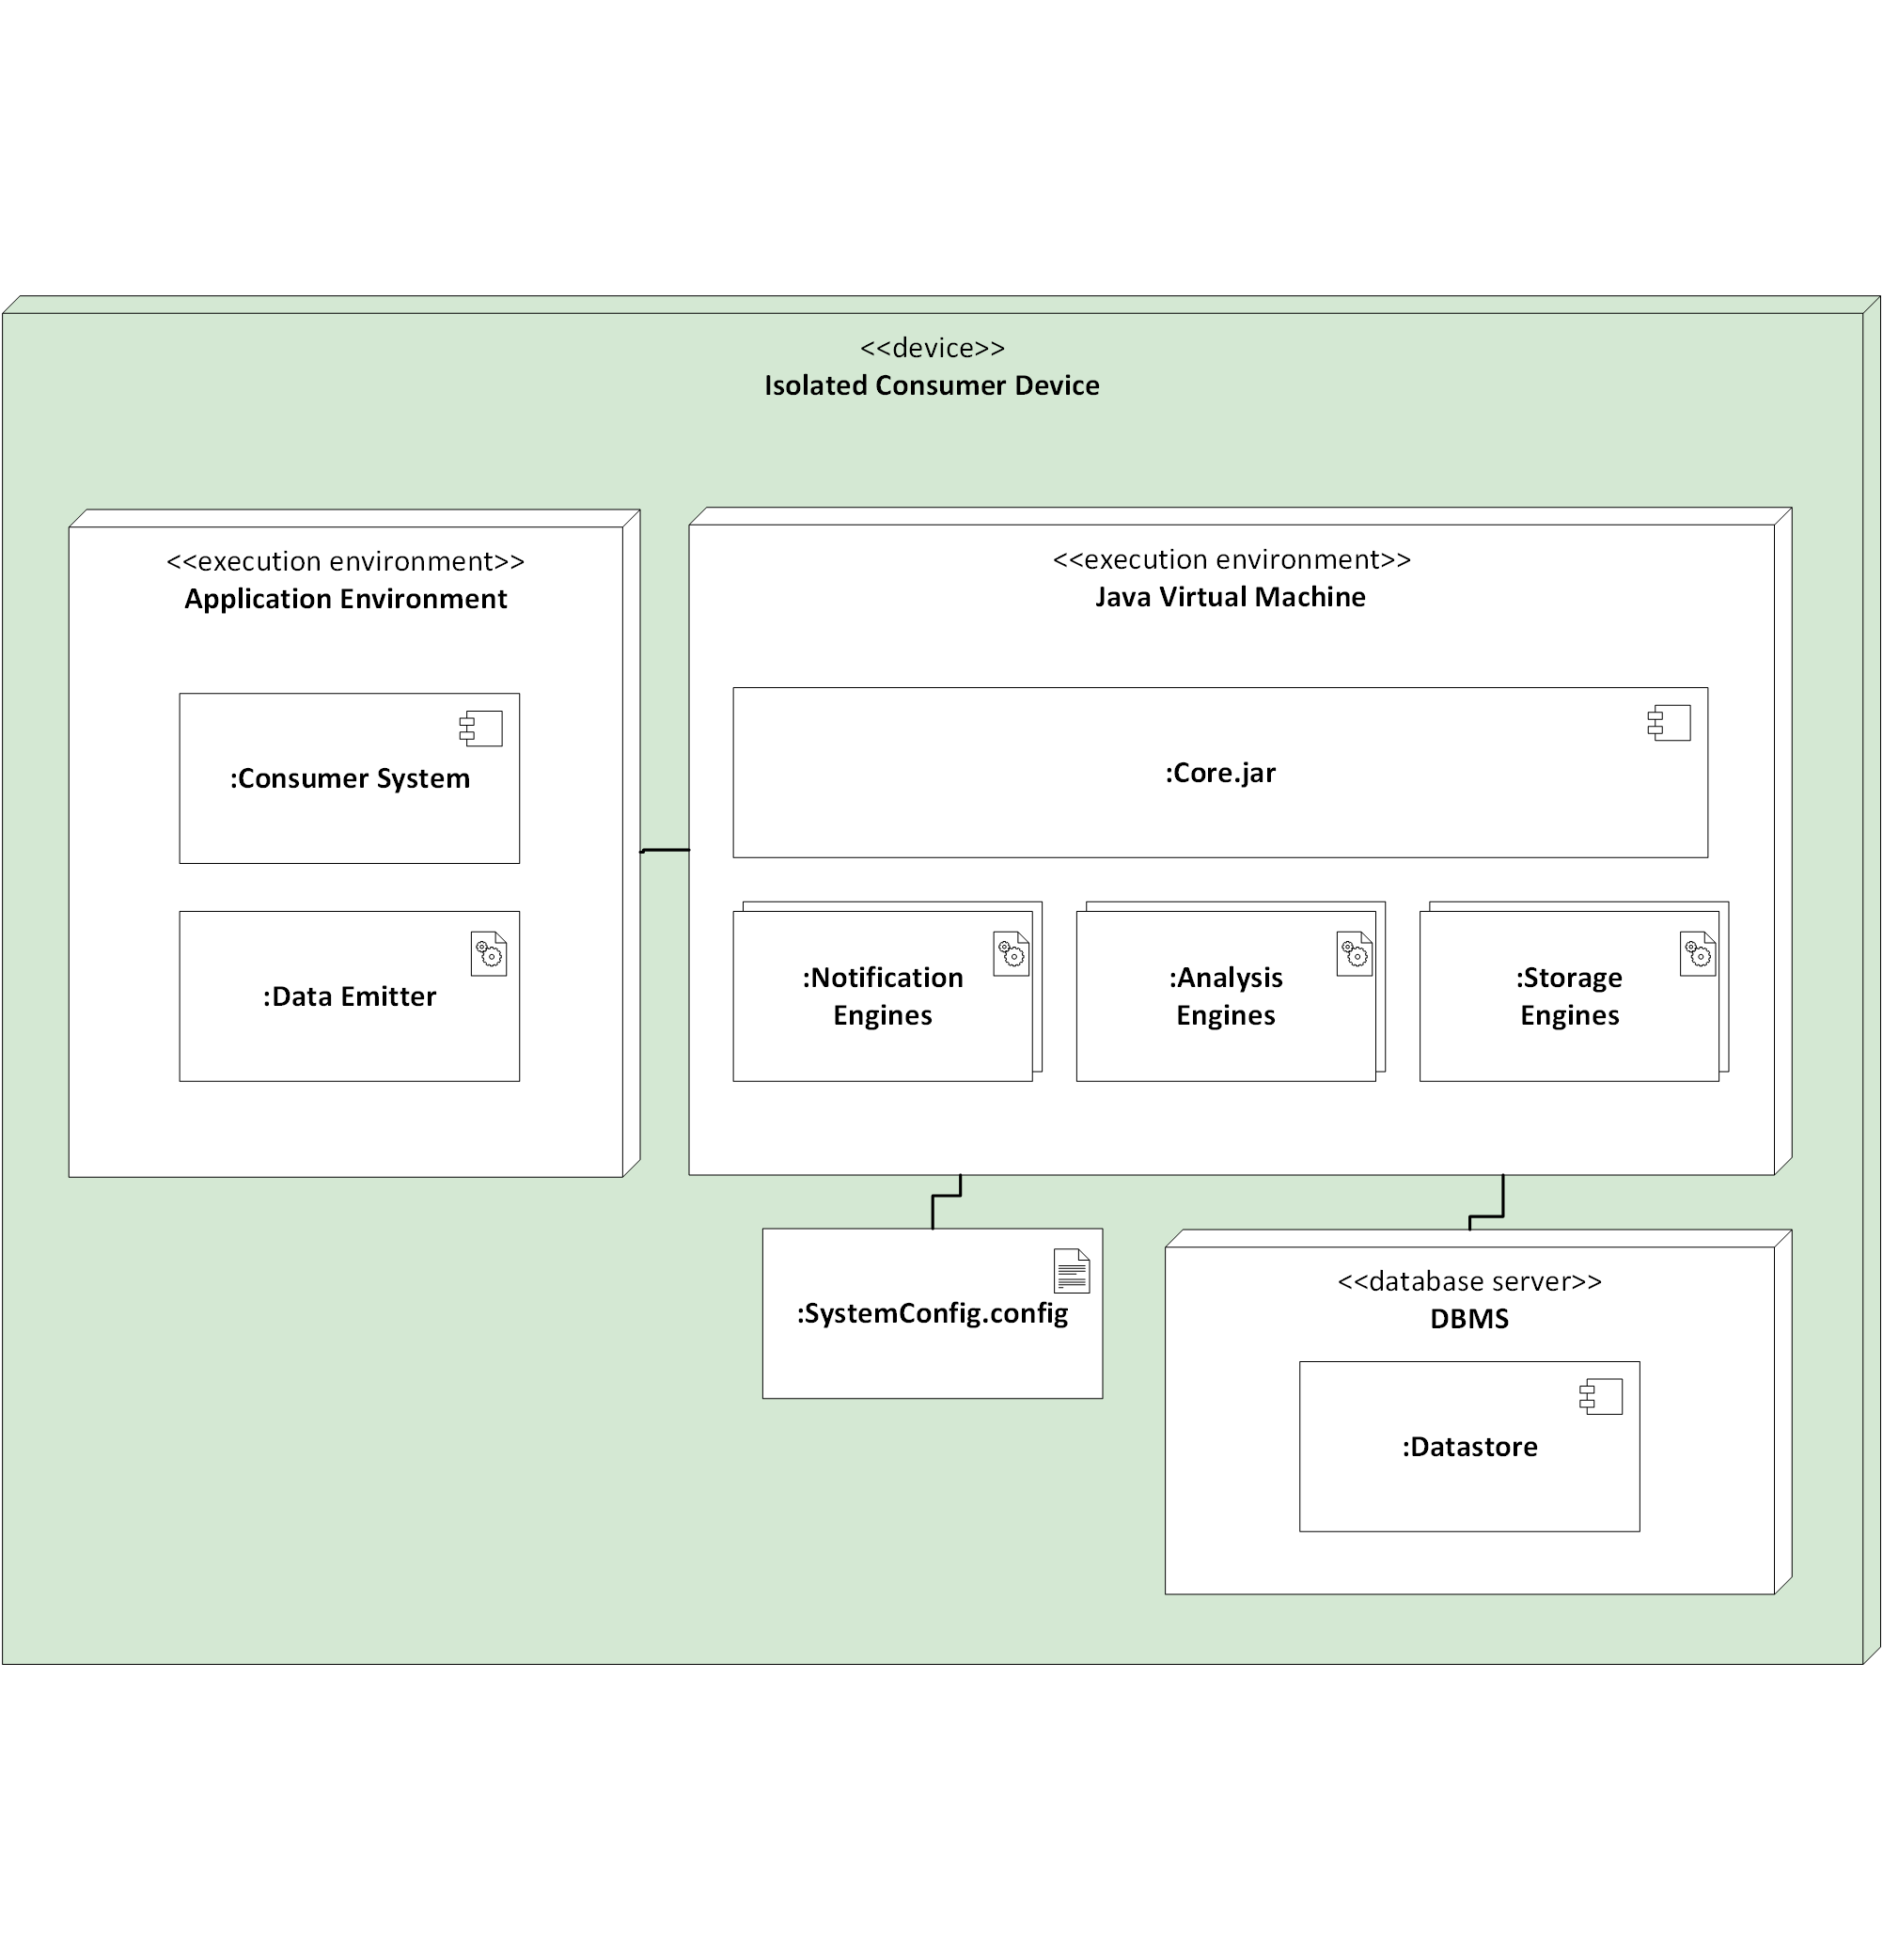
\includegraphics[width=0.8\textwidth]{images/Isolated.png}
  \caption{A deployment of the HUMS in which all components are allocated to an isolated device which is under the Consumer's control.}
  \label{fig:deployisolated}
\end{figure}

\begin{figure}[htp]
  \centering
  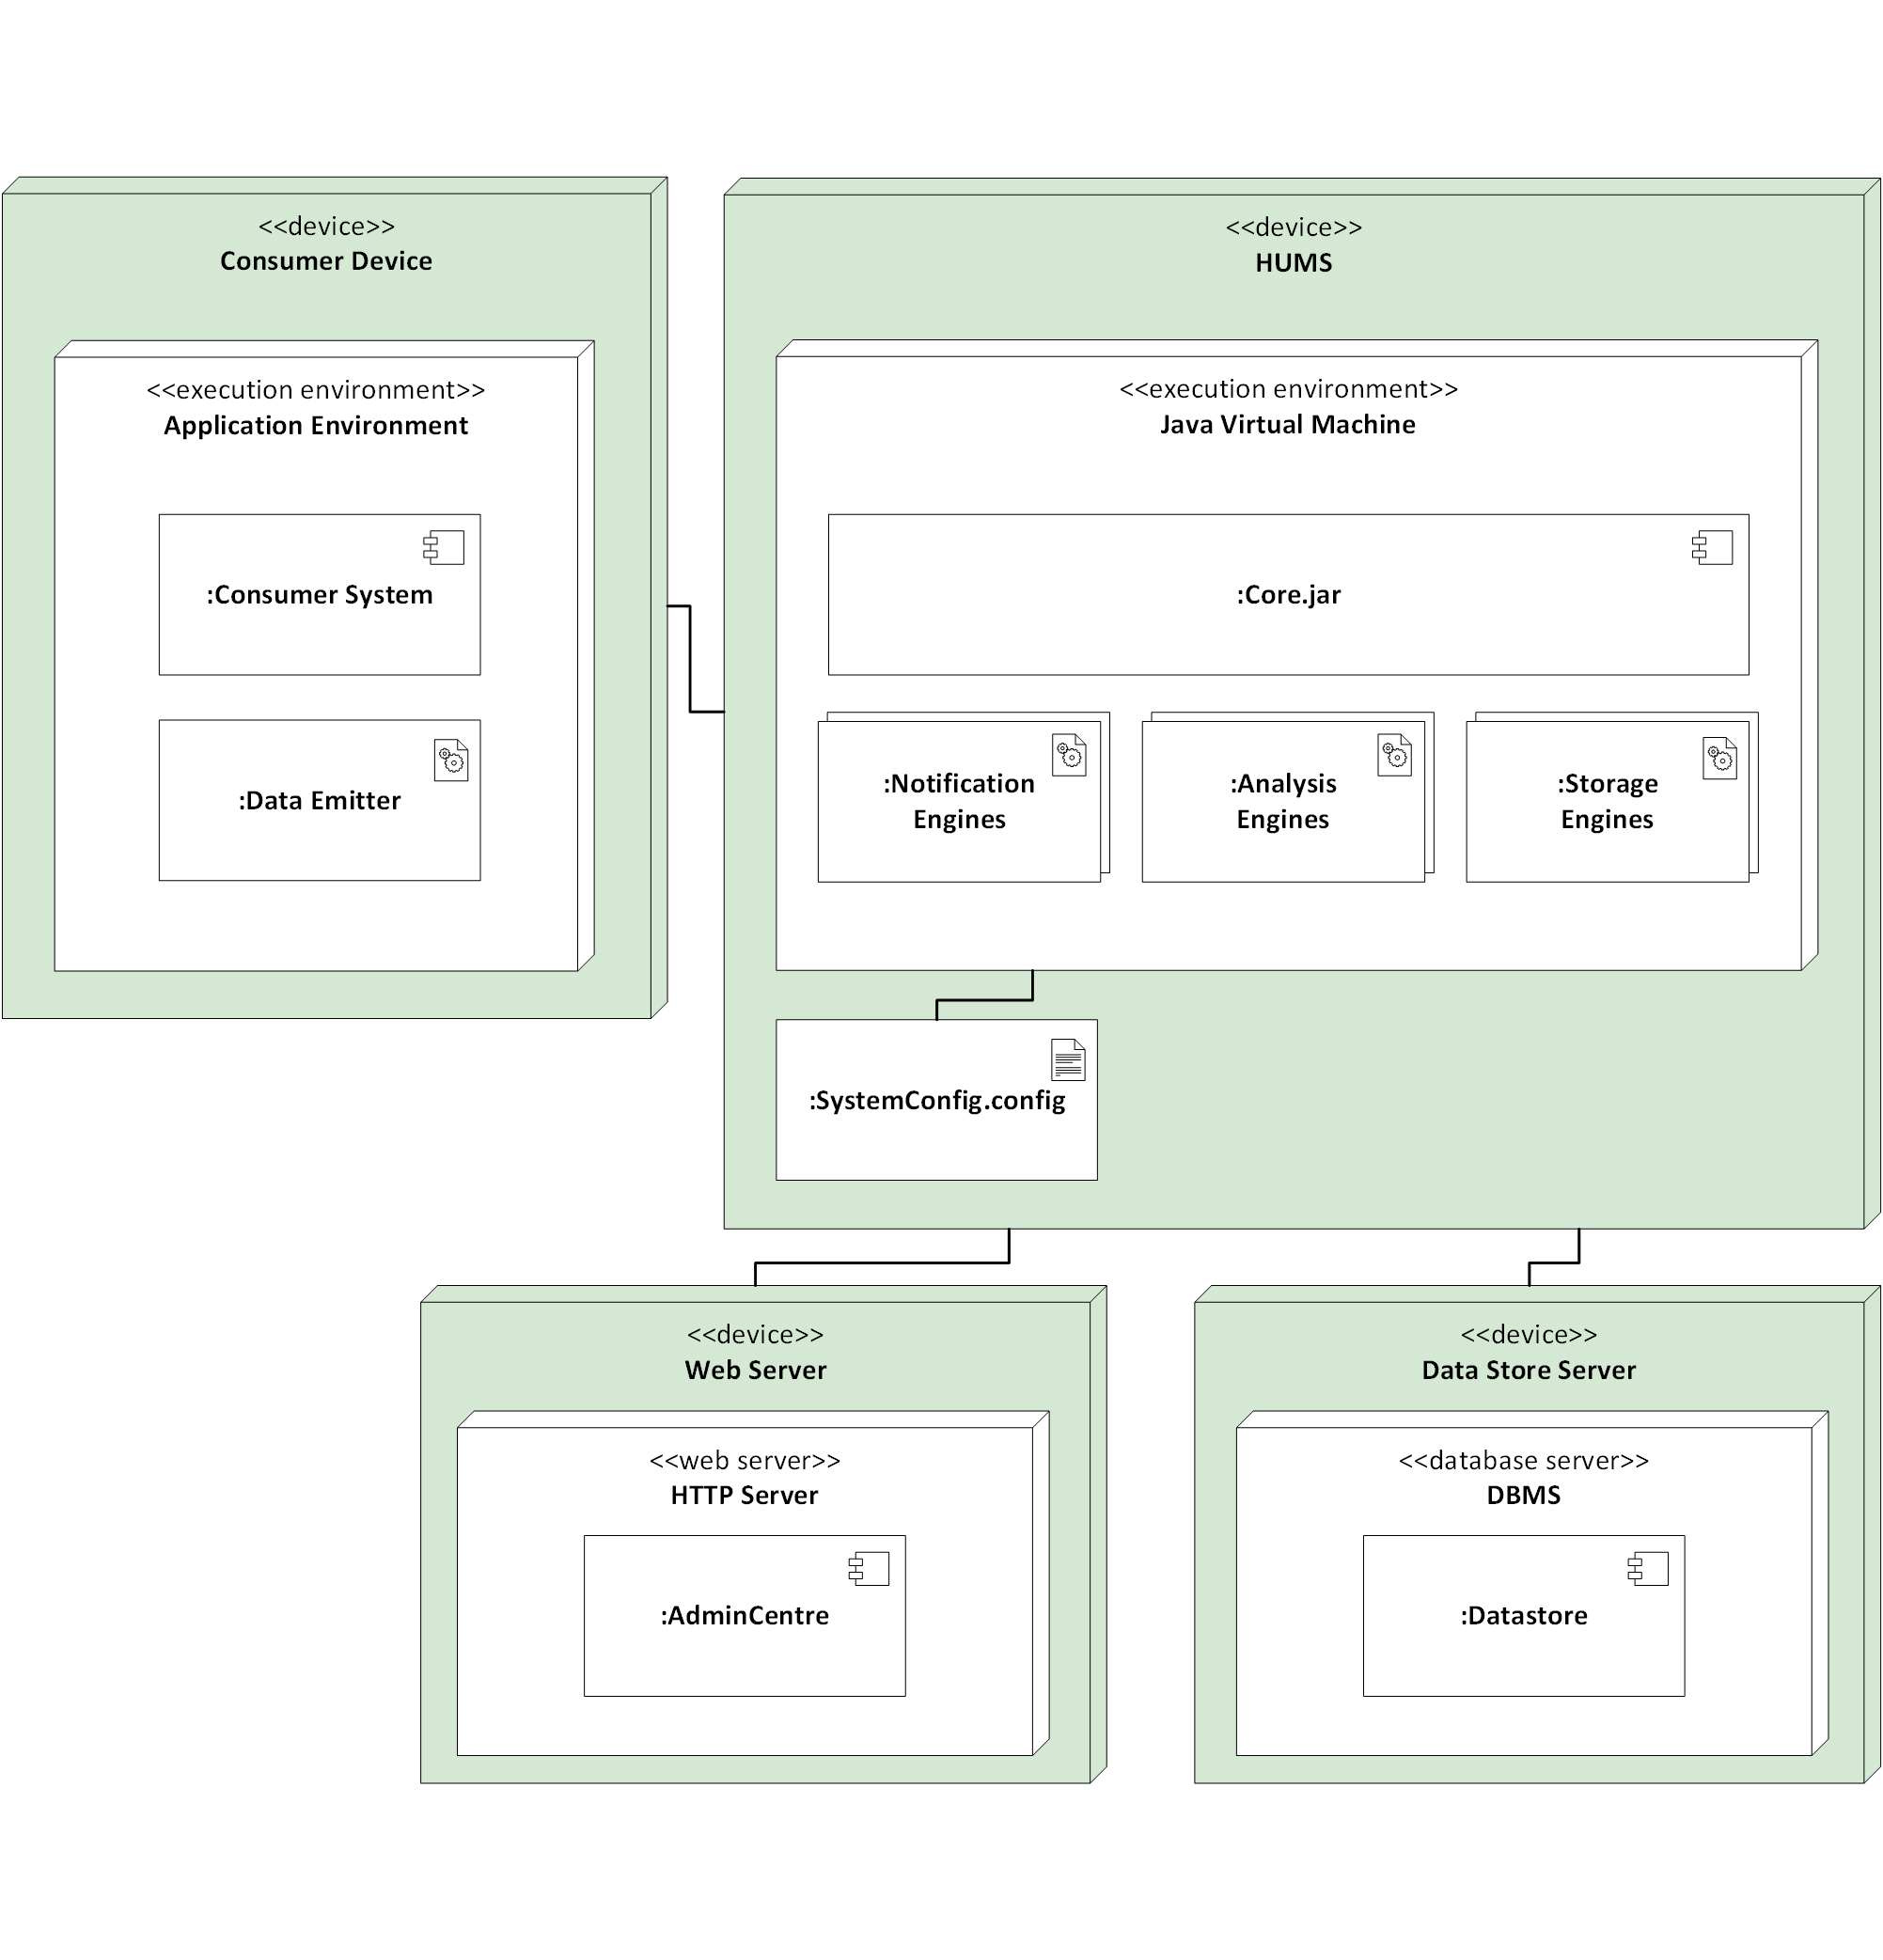
\includegraphics[width=0.8\textwidth]{images/Distributed.png}
  \caption{A deployment of the HUMS in which components are distributed amongst a number of devices which are all under the Consumer's control.}
  \label{fig:deploydistributed}
\end{figure}

Figure~\ref{fig:deployscaled} shows how the HUMS capacity can be scaled up to support many Consumer systems. Due to the modular design of the system, various components can be allocated to multiple devices and scaled independently. Many Consumer devices may communicate with the HUMS at any time. To support an increased capacity, load balancers may be introduced to divide the load amongst a number of Cores. This architecture supports dynamic scaling, in which additional Cores are allocated when necessary. Figure~\ref{fig:deployhumsaas} shows how these architectural qualities allow the HUMS to be deployed as a service (SaaS). The SaaS allocates Cores according to Consumer demand, allowing the Consumer systems to emit data without any knowledge of how these Cores are allocated. A web interface is provided for Consumers to configure their HUMS instances.

\begin{figure}[htp]
  \centering
  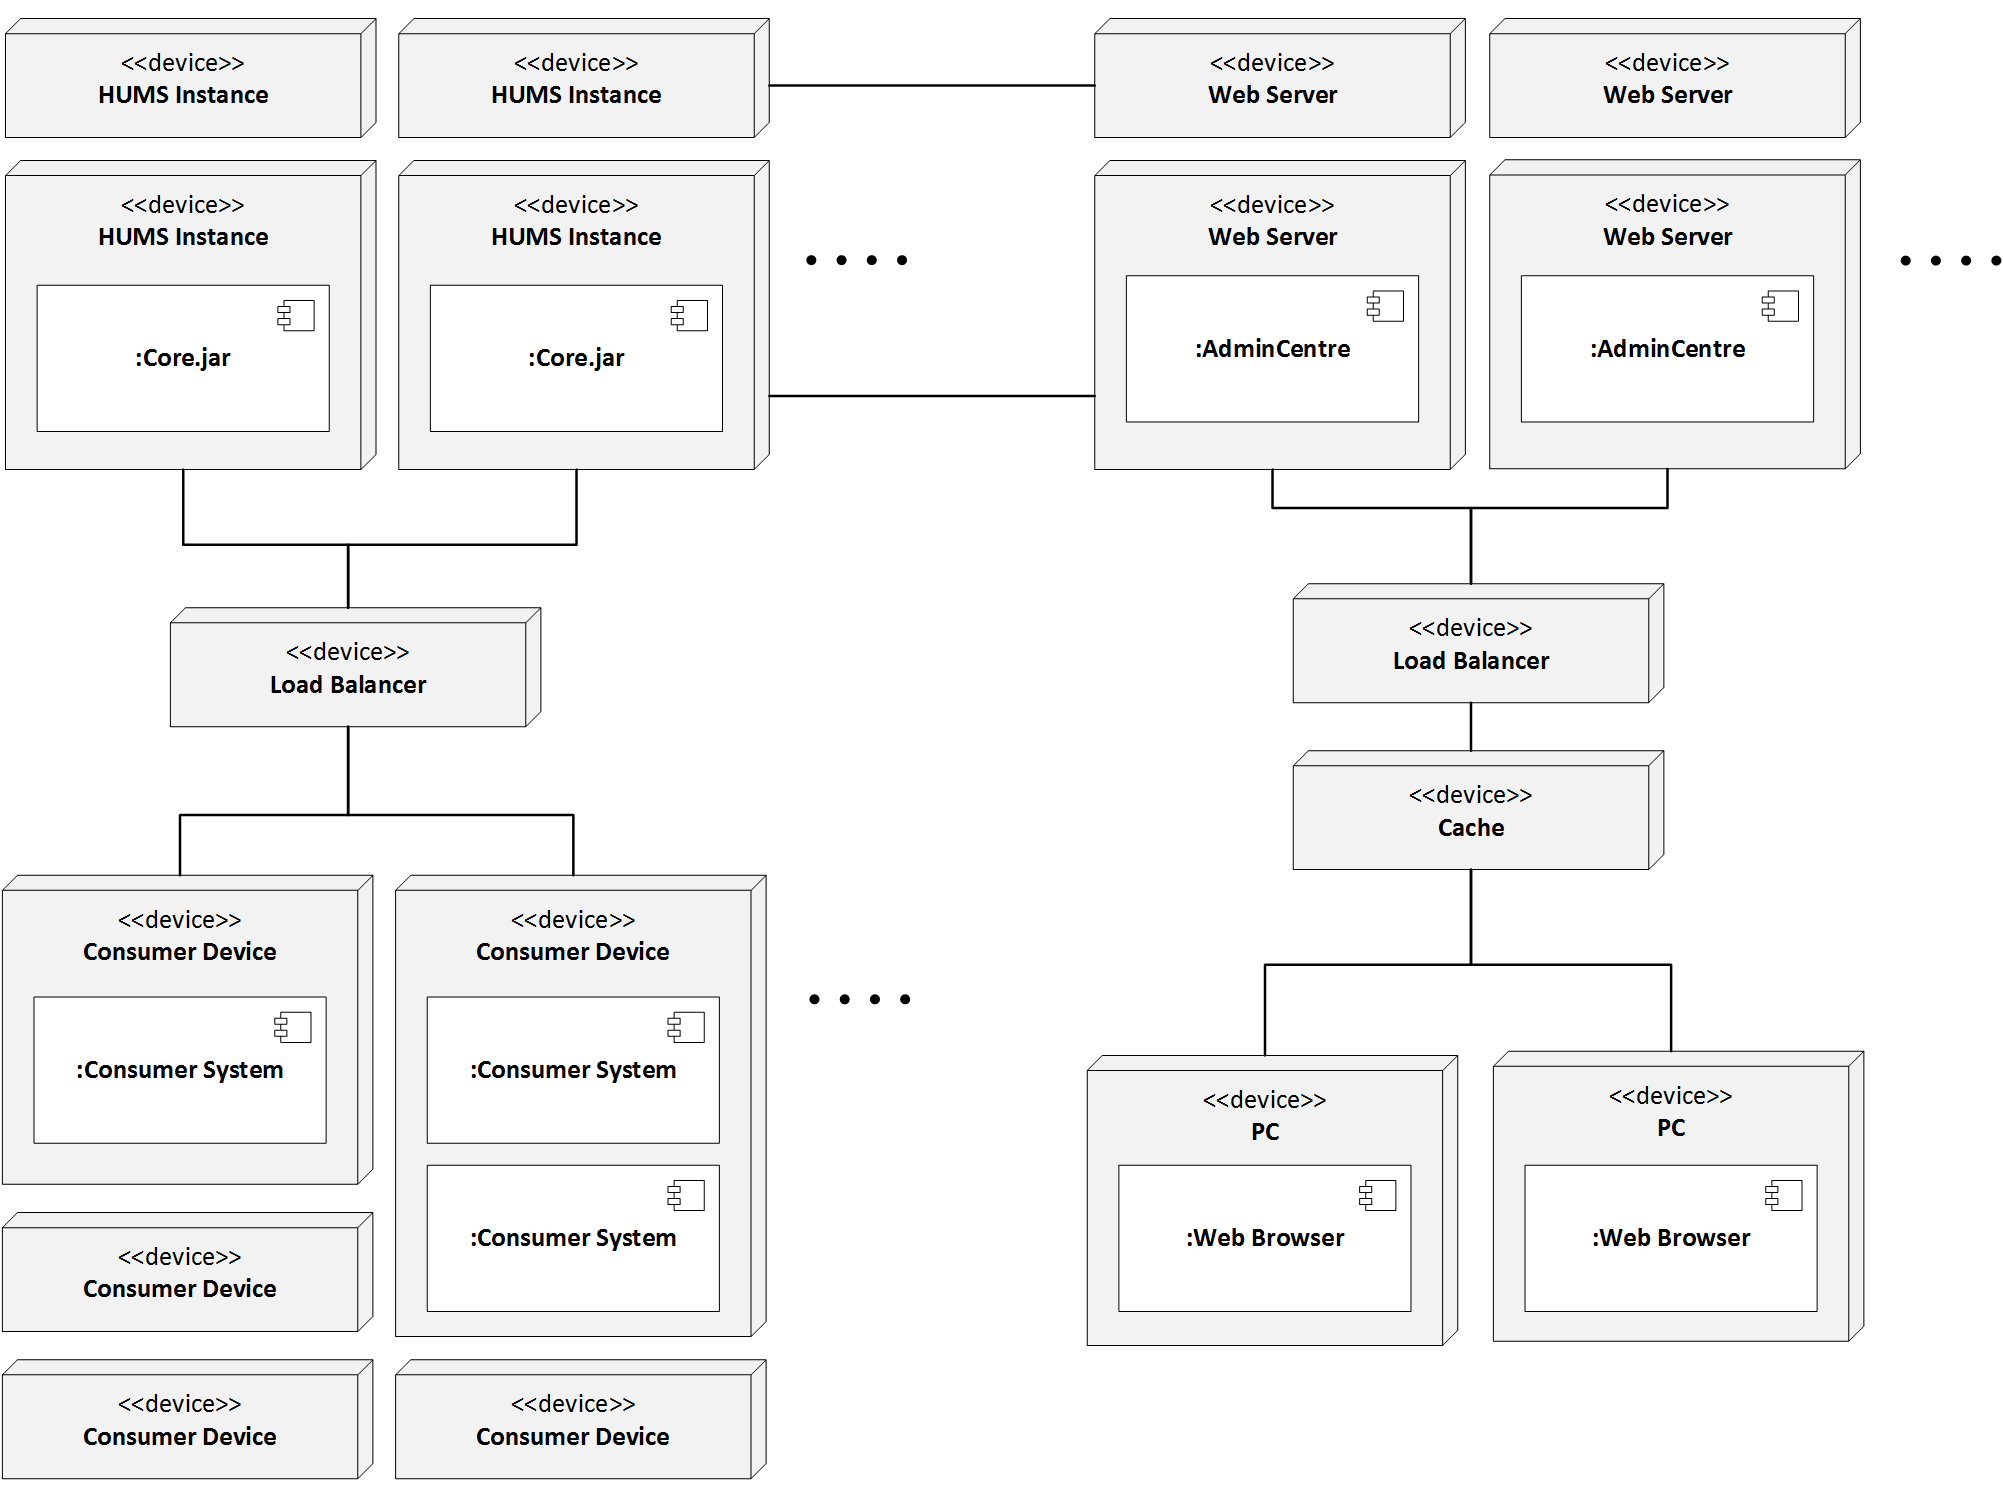
\includegraphics[width=0.75\textwidth]{images/Scaled.png}
  \caption{The HUMS components are easily scaled to allow for an increased load capacity.}
  \label{fig:deployscaled}
\end{figure}

\begin{figure}[htp]
  \centering
  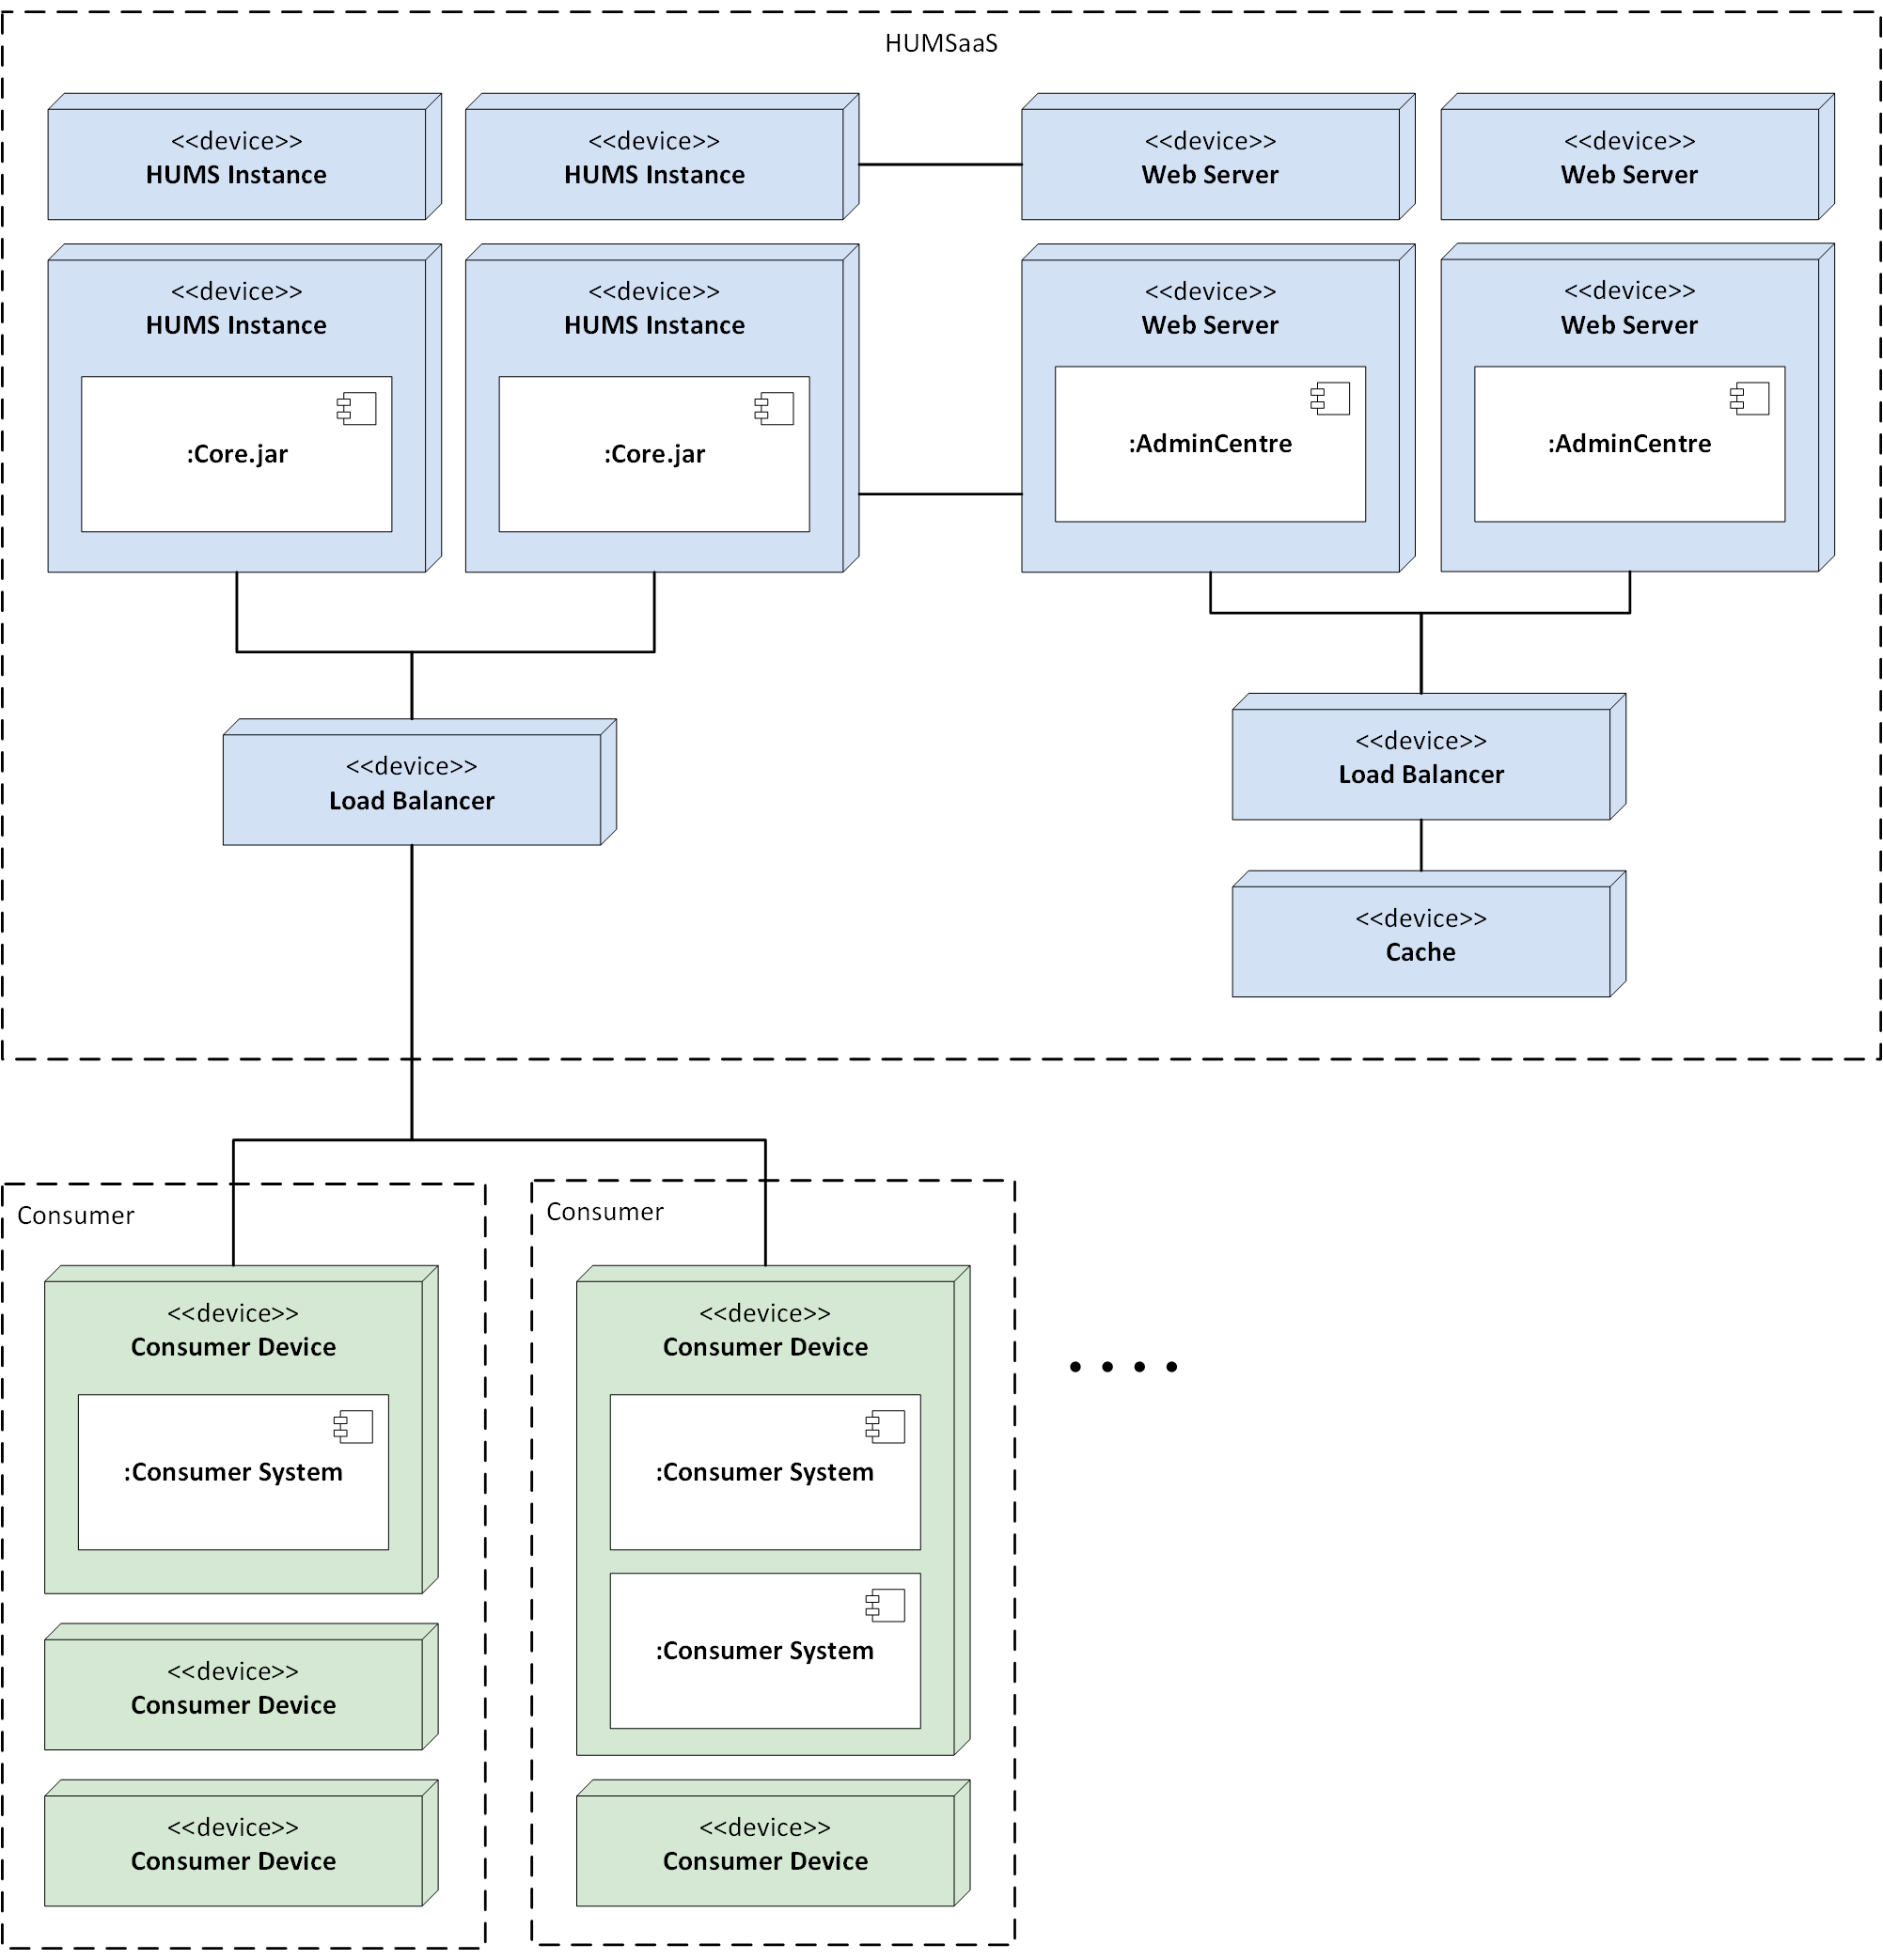
\includegraphics[width=0.75\textwidth]{images/HUMSaaS.png}
  \caption{The HUMS can be deployed as a service to which Consumer's can subscribe in order to analyse data emitted by their devices.}
  \label{fig:deployhumsaas}
\end{figure}

For the purposes of demonstration, the HUMS prototype has been configured to support a number of Data Emitters, with various engines for each, and to store data in a variety of Datastores. Most components are deployed to a single device, while one Data Emitter is deployed to an Android smartphone and three Datastores are provided by cloud services. The complete deployment for demonstration is shown in Figure~\ref{fig:deploydemo}.

\begin{figure}[ht]
  \centering
  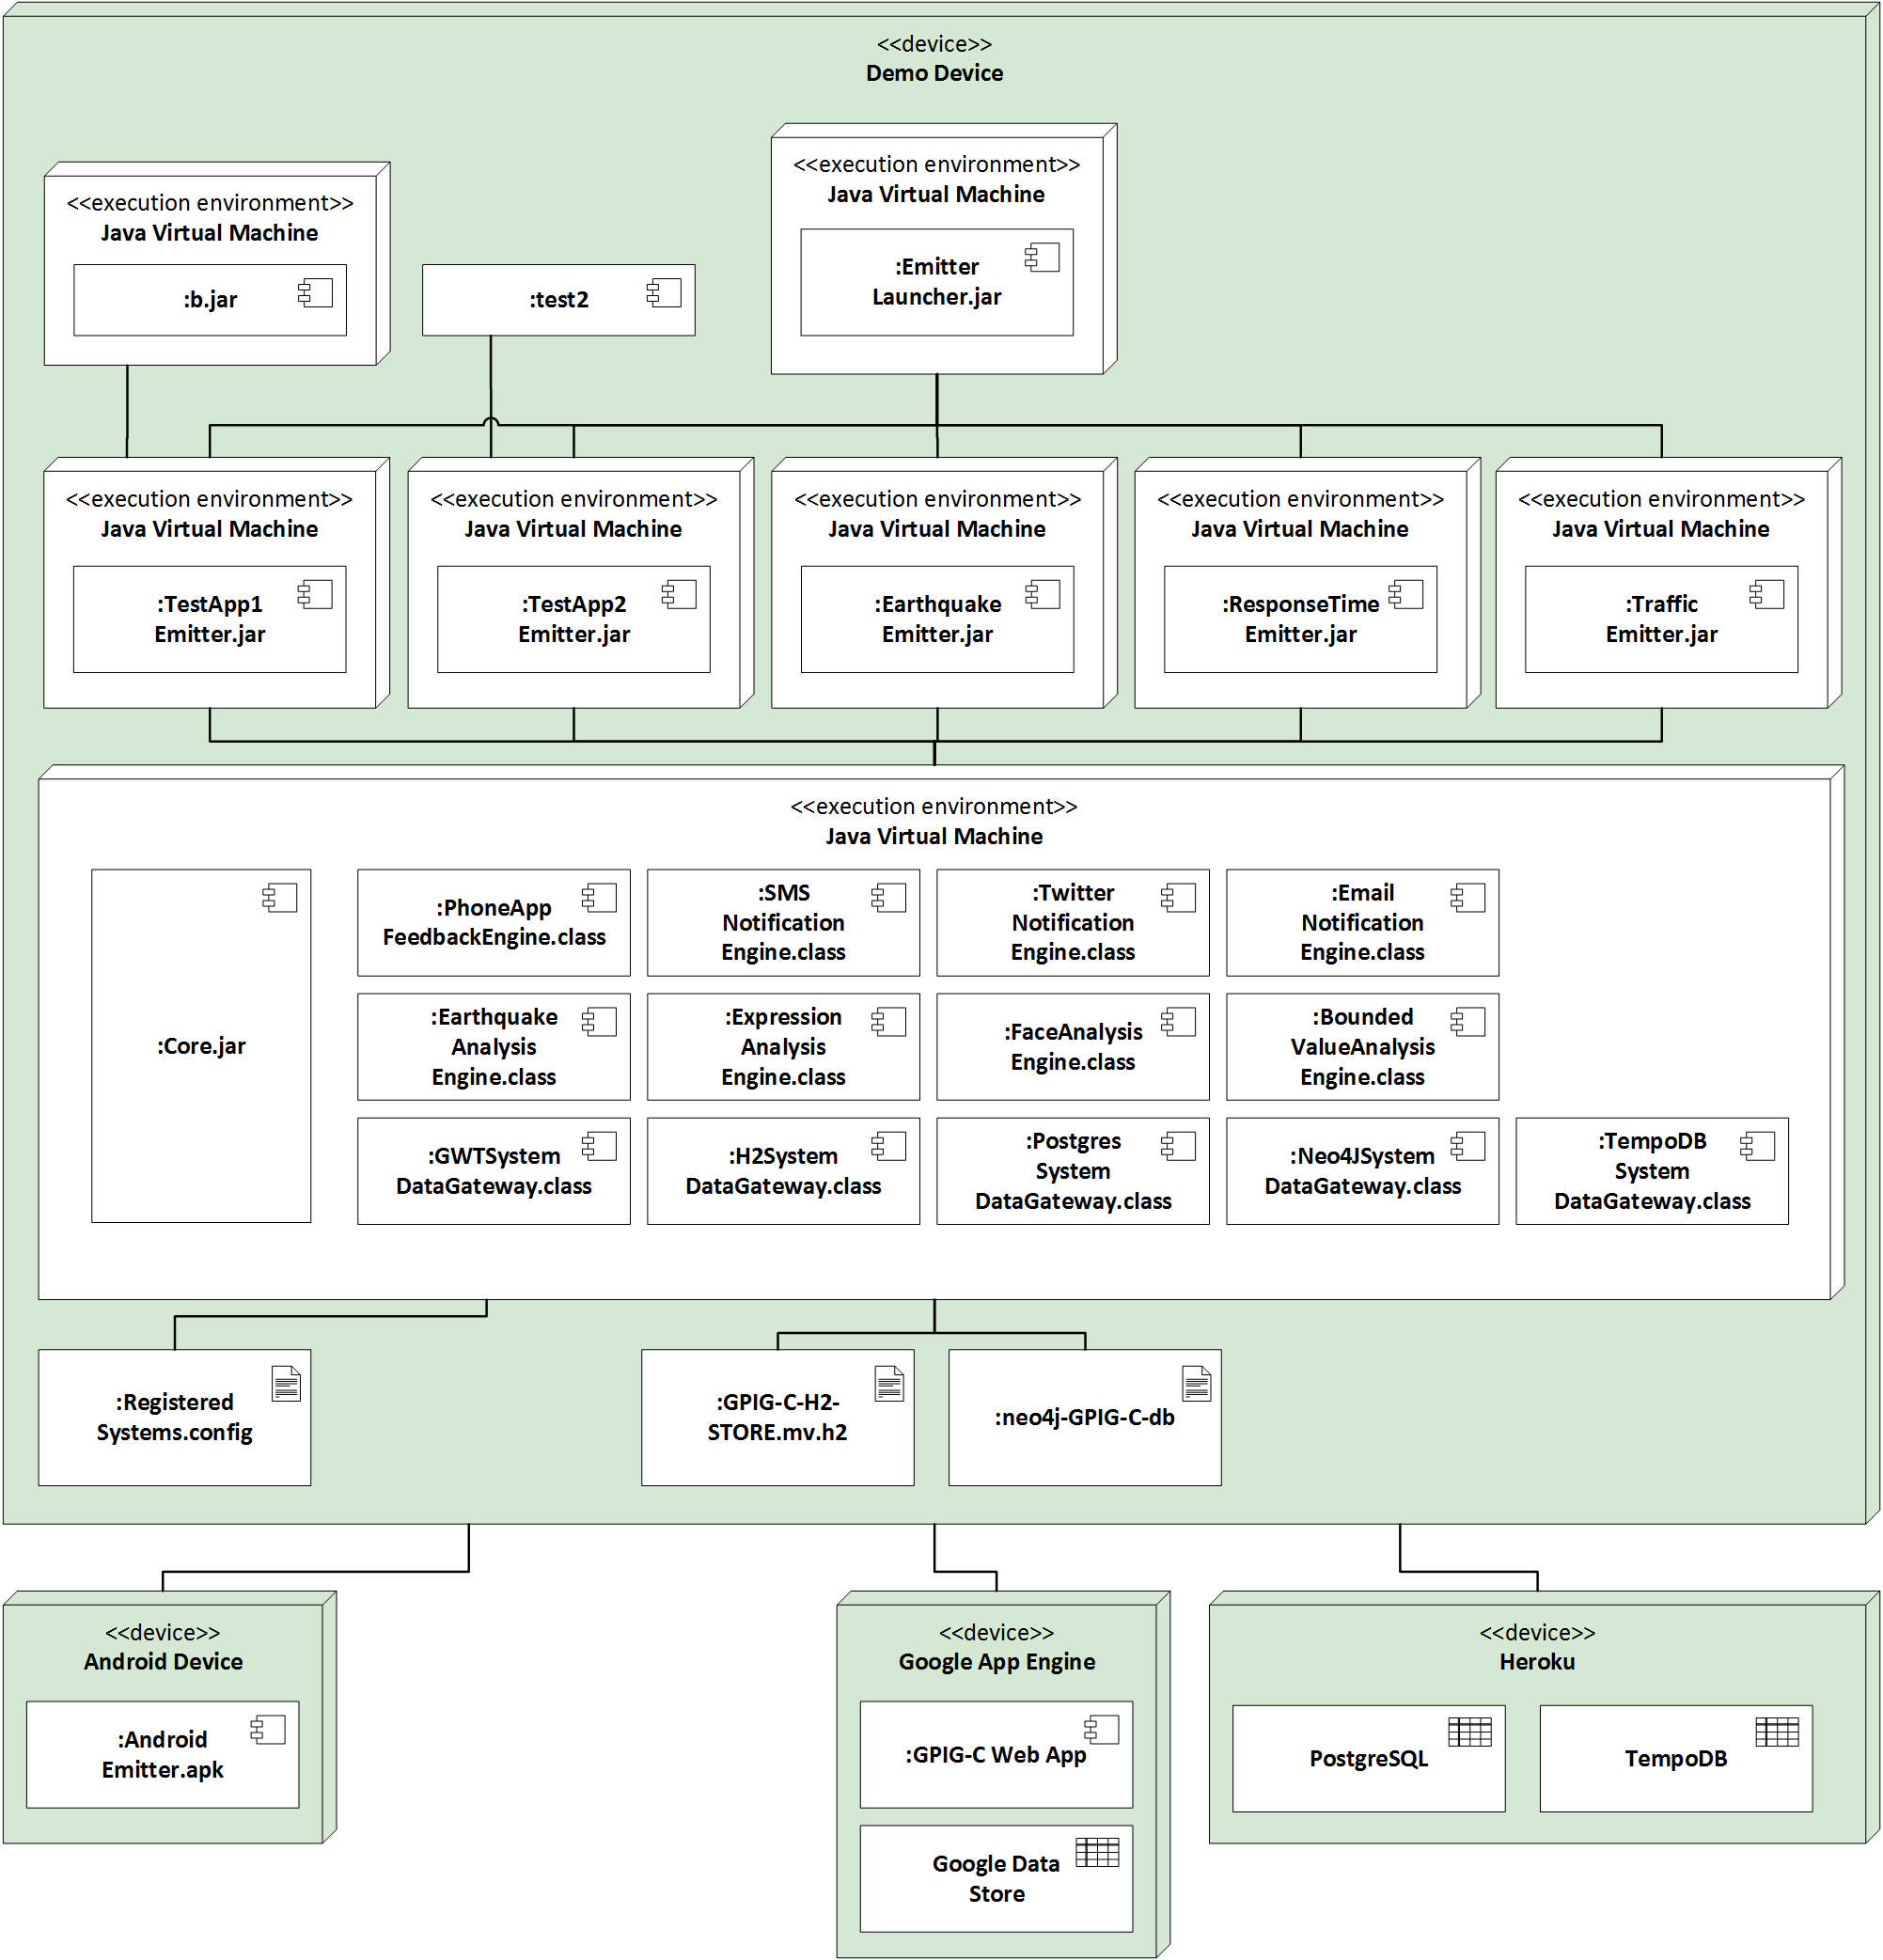
\includegraphics[width=0.8\textwidth]{images/Demo.png}
  \caption{A concrete deployment of the HUMS used for demonstration purposes.}
  \label{fig:deploydemo}
\end{figure}

%-------------------------------------------------------------%
%-------------------DEVELOPMENT-------------------%
%-------------------------------------------------------------%
%   Notes: 					         	 %
%  	- Reference risks constantly, lots and lots	 %
%	- Reference requirements and scenarios 	 %
%-------------------------------------------------------------%

\section{Implementation}
\label{sec:dev}
In this section, the prototype implementation that has been developed is described in detail. This begins with an overview of the implementation at the time of the Interim Report and then covers any changes that have been made. During this development, our team was structured as described in the previous report. However, we did have to modify the project plan slightly to accommodate other commitments. Luckily, we had considered this in risk \emph{R.2} and had appropriate contingency and mitigation strategies in place, meaning the impact was minimal.

\subsection{Interim Implementation Summary}
\label{sec:interim_summary}
At the time of submitting the Interim Report, we had implemented the basic functionality of our Core, with data being sent through the Input Interface and controllers managing engines. However, we did not have dynamic class loading and the Consumer was not able to add classes at runtime. The Consumer was able to create their own engines, but would be required to rebuild the HUMS in order for any additions to take effect.

We had created a Data Emitter for the first test application provided by the Customer, and an additional Data Emitter monitoring earthquakes. We had also implemented a Datastore using Google App Engine, and had created a basic analysis engine which computed the mean of the latest data for a System and created an \texttt{Event} if that mean was outside predefined bounds. The parameters used for analysis and to determine system sensors were hard-coded as the configuration file functionality had not yet been implemented. An \texttt{EmailNotificationEngine} had also been created which sent emails to a defined address. 

We had developed a low fidelity Admin Centre with static HTML and JavaScript, which had been designed appropriately but had no real functionality.

Overall, our interim solution was a low fidelity end-to-end solution, but did not meet all of our requirements and was not impressively tailorable or configurable. 

\subsection{Core Development}
\label{sec:core}
 %giving fully dynamic configurability, that is, it is configurable both at runtime and compile time.
 % and then load the class file at runtime or compile time to extend or modify the default HUMS to meet their needs.
 
The HUMS Core is the main application controlling the behaviour and functionality of the HUMS. It receives Client data from Data Emitters, stores that data, and then passes it to appropriate analysis engines which can create \texttt{Event} objects for the Core to pass to relevant notification engines.

\texttt{Controller} objects are used to dynamically load and manage the three different engine types: analysis, notification, and storage engines. The addition of dynamic class loading increases the configurability and modifiability of the System by allowing the new engines to be added both at runtime and compile time, making our HUMS fully dynamic.

In addition, the Core now automatically detects when new files are added to the folder they are loaded from and refreshes the System. This means that from the Consumer's perspective they merely have to place their class into the correct folder to load it, increasing the HUMS's usability.

Several example applications provided with our HUMS are described in this report. These implement standard interfaces provided with the HUMS Core, one for each of the three engine types. The Customer and Consumer can therefore easily extend and tailor the System by creating their own engines to meet their needs.

The Consumer system and Sensors monitored by a particular HUMS instance and how they will be monitored is defined using a JSON configuration file. An example of the format of this file is displayed in Figure~\ref{fig:configFiles}, showing the definition of a particular Consumer system with a System ID, Sensor IDs, parameters, and which engines the system uses. A System configuration file (\texttt{*.config}) is loaded into the Core by the Consumer before it is run. Changes to configuration files can be made manually through a text editor or in a more user-friendly manner through the Admin Centre.

\begin{figure}[tbp]
\begin{lstlisting}[language=json,firstnumber=1]
{
    "Systems": [
        {
            "SystemID": "EarthquakeMonitor",
            "Sensors": [
                {
                    "SensorID": "EQ",
                    "Params": {
                        "LOWER_BOUND": "1.0"
                    }
                }
            ],
            "Engines": [
                "EarthquakeAnalysisEngine",
                "TwitterNotificationEngine"
            ],
            "DatastoreGateway": "Neo4jSystemDataGateway",
            "Reporting": "Map"
        },
        etc...
    ]
}
\end{lstlisting}
\caption{An example of a JSON configuration file used by the HUMS.}
\label{fig:configFiles}
\end{figure}

Any changes made to the System configuration file whilst the HUMS is running are automatically detected by the Core and cause the file to be reloaded allowing the alterations to take immediate effect. This reduces risk \emph{R.5} by ensuring the Consumer cannot forget to reload the file, increasing the usability of our HUMS by improving its learnability.

The Core has also been refactored to load Consumer system parameters to be used by engines from System configuration files. This includes both individual Sensor parameters and System parameters meaning that, for example, analysis can be performed both per Sensor and on the System as a whole, further increasing the tailorability of our solution. The configuration file for a particular instance of the HUMS can be set and modified at runtime or compile time, as it is separate from the codebase, making it very versatile and further improving configurability. 

In addition to the above, we created an optional GUI for our HUMS Core which makes the process of configuring and running our HUMS even simpler. Shown in Figure~\ref{fig:coreGUI}, this GUI allows the Consumer to select the configuration file they wish to use and to start and stop the Core with the click of a button. The GUI also keeps the Consumer informed of what the Core is doing through an integrated console, reporting any errors such as incorrectly formatted configuration files alongside the general status of the Core. The GUI was created using the \emph{Standard Widget Toolkit}~\cite{swt}. This was chosen over other UI libraries such as \emph{Swing} as it uses native widgets, such as buttons and menus, improving the user experience by using components they are already familiar with.

\begin{figure}[ht]
\centering
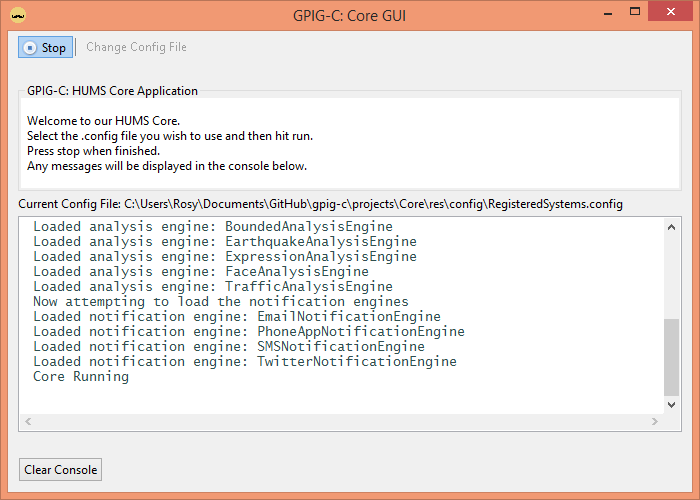
\includegraphics[width = 0.8\textwidth]{images/coreGUI.png}
\caption{A screenshot of the HUMS Core GUI.}
\label{fig:coreGUI}
\end{figure}

A lightweight Jetty server was also added to the Core demonstrating that the Admin Centre can be served from the same system that the Core runs on. This enables further integration between the configuration files and the web interface which now allows these files to be easily administered by both technical and non-technical users, and avoids a custom server having to be manually set up by the Consumer as the process is automated.

\subsection{Sensing}
\label{sec:monitor}
In this section, we describe the applications our HUMS currently monitors. We created six sample Data Emitters for this stage of the project in order to demonstrate the tailorability of our HUMS. These show how the HUMS can integrate with existing applications and APIs, as well as how it can be used with specially-made applications. A Consumer would be able to quickly create a Data Emitter for their own application by using the interfaces provided with our HUMS Core.

\subsubsection{Test Application Data Emitters} 
\label{subsec:tapp}
Part of our task was to monitor the test applications provided by the Customer, treating them as black-box systems. For the first test application, we simply monitored the memory and CPU usage, but for the second we also added swap state, number of threads, last processor it was run on, and working directory. For this we created a process monitoring Data Emitter which is capable of tracking information from a process. This utilises the \emph{System Information Gatherer} (SIGAR) library. SIGAR is a cross-platform library which allows system information and process information to be accessed, without worrying about the implementation that the platform provides for reading that information. The information gathered by these engines is forwarded to the Core for analysis.

\subsubsection{Earthquake and Traffic Data Emitters}
In order to ensure our HUMS is capable of receiving, analysing, and reporting data through various external APIs, we updated our earthquake Data Emitter and added an additional traffic Data Emitter, monitoring real time UK traffic accidents and incidents. The earthquake data (from the U.S. Geological Survey~\cite{us_geo}) is formatted as JSON and the traffic data (from the UK Highways Agency~\cite{ha_traffic}) as XML, which are both standard and commonly used data formats. These two emitters demonstrate the extensiblility of the HUMS as similar additional Data Emitters can easily be created to read data from other sources, which would likely also use the same or similar formats.

\subsubsection{Server Responsiveness}
A common use of existing HUMS implementations is in monitoring the responsiveness of websites and servers, alerting users and staff if the system becomes unavailable. In order to ensure our HUMS was capable of such a task, we implemented a response time Data Emitter which determines the response time of requests to a given website\footnote{thalesgroup.com} and sends this data to the Core for analysis.

\subsubsection{Emitter Launcher}
For demonstration purposes, and to make our prototype easier to test and use, we created an \emph{Emitter Launcher} which simplifies the process of running our desktop Data Emitters by allowing the individually packaged Data Emitters to be simultaneously run from a single application using a GUI. A screenshot of this GUI is shown in Figure~\ref{fig:launcherGUI}, which has again been created using the \emph{Standard Widget Toolkit} \cite{swt}, meaning native components can be used.
 
\begin{figure}[ht]
\centering
\includegraphics*[width=0.8\textwidth]{images/launcherGUI.png}
\caption{A screenshot of the Emitter Launcher GUI.}
\label{fig:launcherGUI}
\end{figure}

\subsubsection{Android Mobile Application}
To explore the possibilities surrounding monitoring remote systems over a network, we created an Android application with three test systems allowing us to demonstrate that our HUMS is capable of this. Screenshots of the Android application are shown in Figure~\ref{fig:android}.

The first system simulates a car monitoring application, allowing users to select values for a number of Sensors and then push them to the remotely-based Core. In a real system, the user would not set the values or manually push them---it would be automatic---however, we have chosen to manually update the data for the purposes of demonstrating the functionality.

The second system is a phone battery monitoring application, which allows the user to define how long they would like to use their mobile device for and based on the given battery life, uses the HUMS to determine which services can stay on in order for this target to be met. The HUMS feeds back into the phone system, toggling services as necessary to balance device functionality and battery usage. This system was designed to show how our HUMS is capable of monitoring a system, and feeding information back to alter the system's behaviour in response to the information it collects.

The final system performs face recognition, collecting face data using the built-in device camera, forwarding that data to the HUMS for analysis. This system was included to show how our HUMS allows for fast, complex, and specific data analysis, in this case using computer vision algorithms, in order to show that risk \emph{R.8} has not been realised. 

\begin{figure}[ht]
\centering
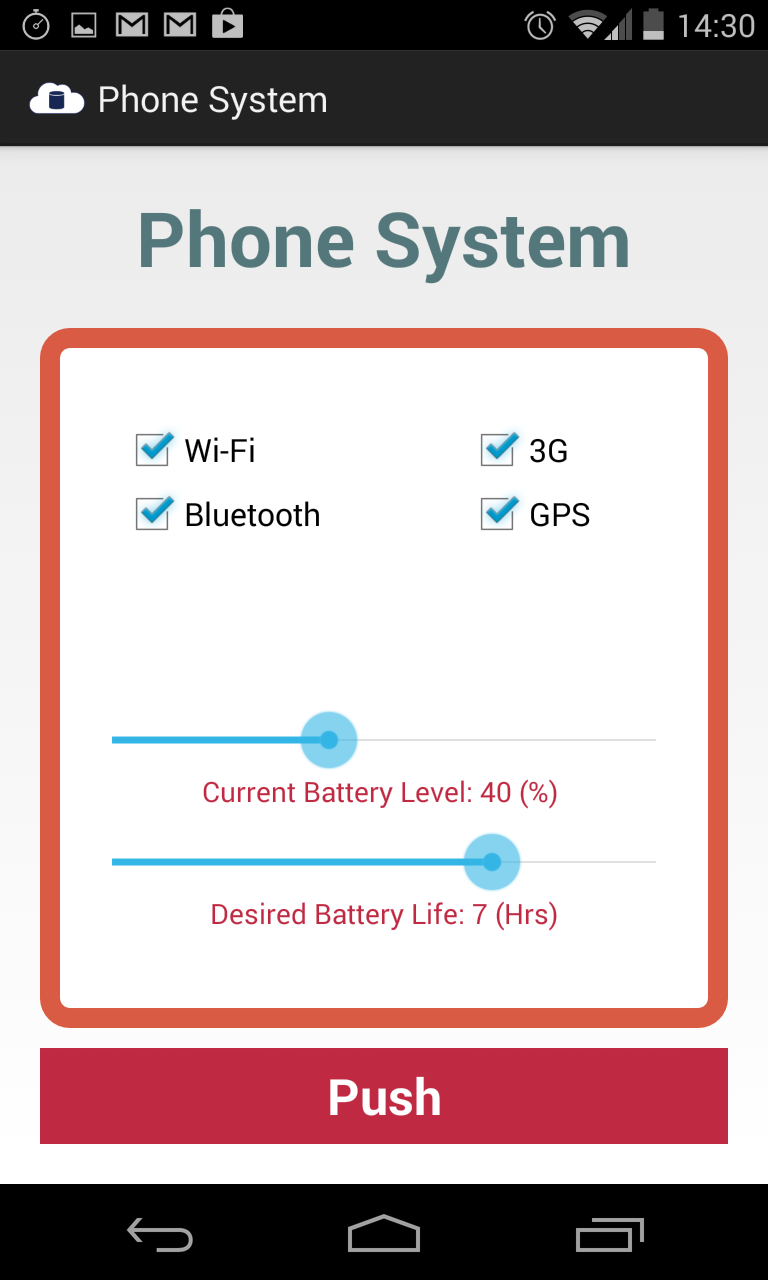
\includegraphics[width=4.3cm]{images/phoneApp.png}
\hspace{0.5cm}
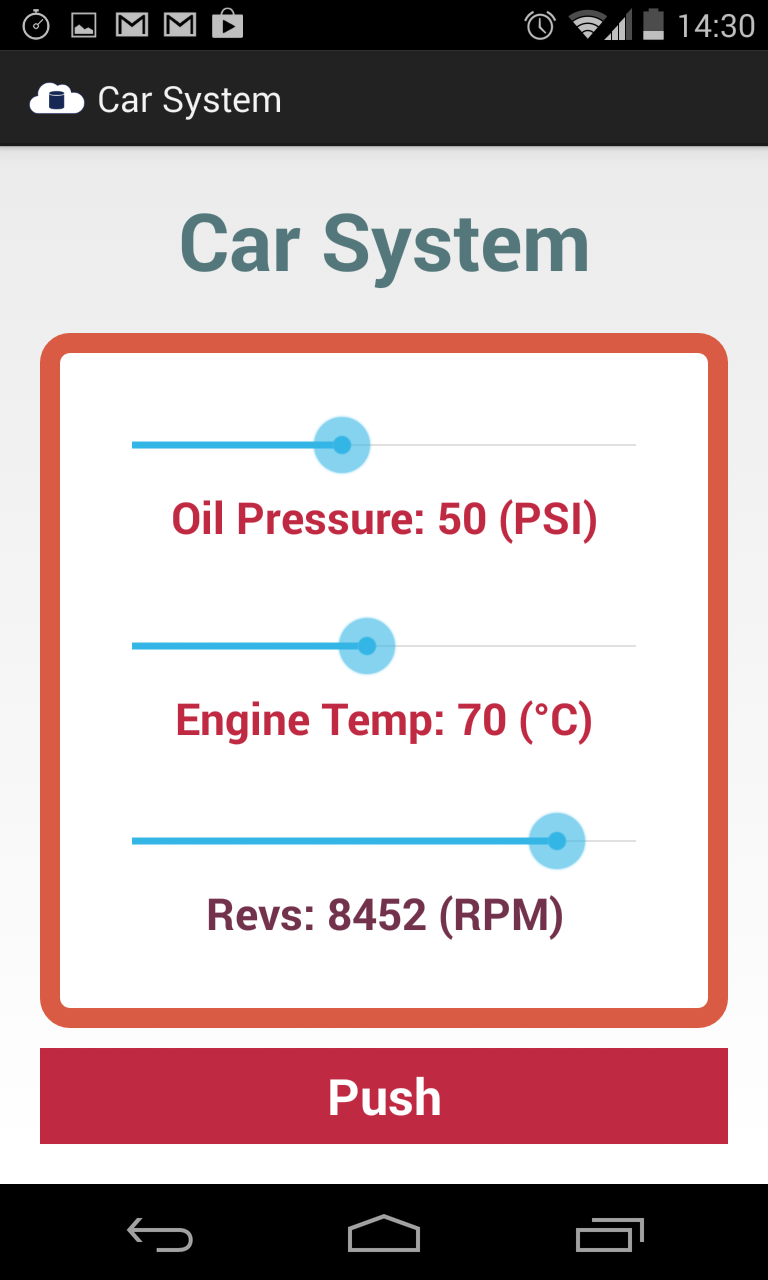
\includegraphics[width=4.3cm]{images/carApp.png}
\hspace{0.5cm}
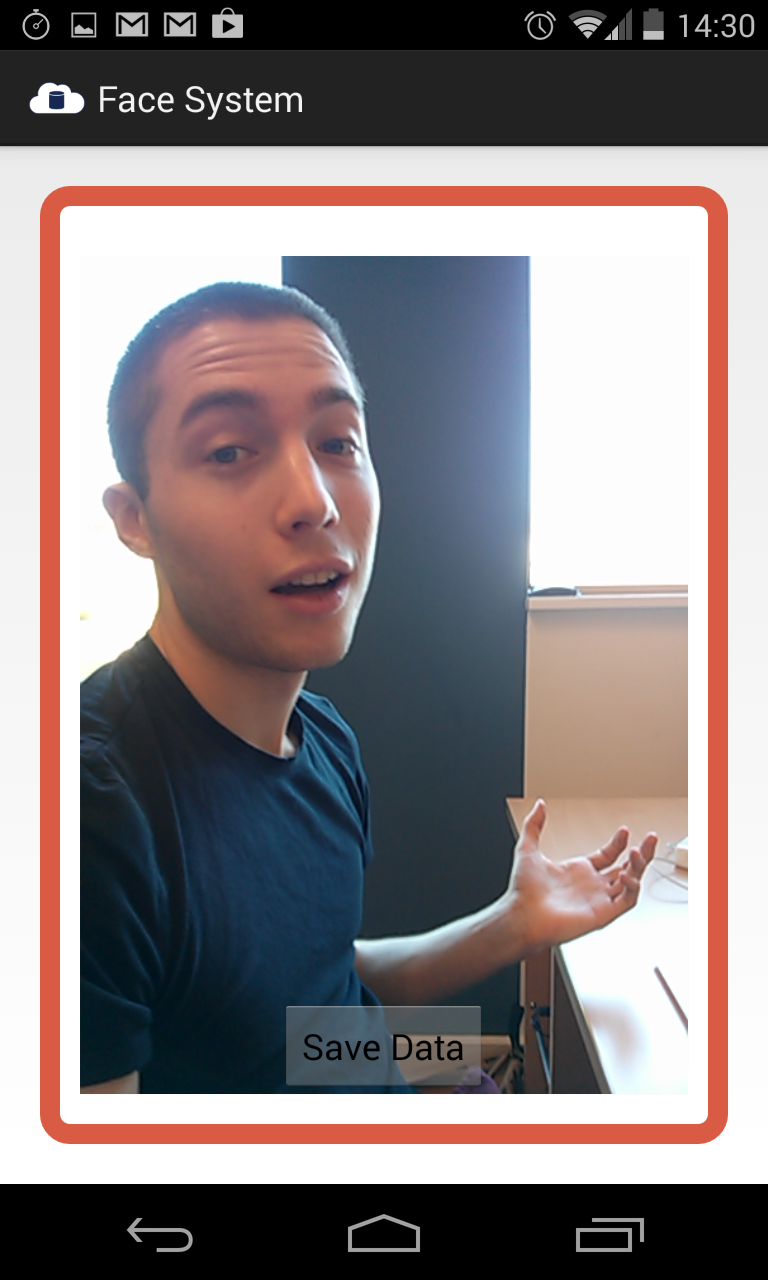
\includegraphics[width=4.3cm]{images/faceApp.png}
\caption{Screenshots of the Android mobile application, showing each of the three subsystems.}
\label{fig:android}
\end{figure}

\subsection{Storing}
\label{sec:store}
This section describes how our HUMS implementation stores data. Our HUMS provides a generic \texttt{SystemDataGateway} interface which can be implemented for a variety of Datastores, allowing for polyglot persistence. To demonstrate this, we created five sample implementations interfacing with a range of popular storage solutions, including: \emph{Google App Engine}, \emph{PostgreSQL}, \emph{Neo4j}, \emph{TempoDB} and \emph{H2}. This was done to show how our System does not force the Consumer to conform to a particular data schema or data storage technology. In fact, the Datastores registered to our sample systems can be modified in the configuration file without any errors occurring. This method increases the overall tailorability of our solution whilst addressing risks \emph{R.7} and \emph{R.8}. The remote Datastores used in our implementation were chosen as they allow \emph{NFR.9--10} be achieved.

Prepared statements were used where possible in the Datastore implementations, being compiled once and then reused, leading to significant gains in performance. Prepared statements also offer improved security against SQL injection attacks, with all user input being treated as data, rather than as part of the queries, and thus not altering the characteristics of data queries.

\subsubsection{Google App Engine Storage}
\emph{Google App Engine} is a popular cloud based Platform as a Service (PaaS) solution, which is used to deploy applications and manage data. We have chosen to use this as part of our implementation to demonstrate how our HUMS can easily interface with a remote NoSQL datastore. We did this by creating and hosting a simple web-based application on \emph{Google App Engine}, and then communicating with it using a \texttt{SystemDataGateway} object which performed the relevant HTTP requests.  

\subsubsection{PostgreSQL Storage}
\emph{PostgreSQL} is a prominent relational database management system, which is queried using SQL and is ACID compliant. We included this storage engine in order to show how our HUMS can interact with a remote SQL Datastore. To implement this we created a \emph{Heroku} web application, which included a \emph{PostgreSQL} database, and communicated with it from a \texttt{SystemDataGateway} object, again using HTTP.

\subsubsection{H2 Storage}
For real-time applications that require high performance and low response times, a local \emph{H2} instance is offered. \emph{H2} is a Java library that implements a simple, self-contained and server-less transactional SQL database. \emph{H2} can be run in embedded or server mode; its small storage footprint of $1.5$~MB and low memory usage make it ideal for use in resource constrained environments. 

\subsubsection{Neo4j Storage}
To demonstrate that our HUMS can work with a distributed Datastore, running on a local cluster or machine, we included a \emph{Neo4j} storage engine. \emph{Neo4j} is a graph database, where data is stored in nodes connected by types and directed relationships. This allows for a more interesting analysis which can take advantage of the relationships between nodes. It also allows for easy distribution and sharding across machines, with each Consumer system creating a distinct sub-graph, meaning performance is increased. An example of data stored by Neo4j is presented in Figure~\ref{fig:neo4j}.

\begin{figure}[ht]
\centering
\includegraphics*[width=0.8\textwidth]{images/neo4j.png}
\caption{A graphical representation of a snapshot of the Neo4j Datastore contents.}
\label{fig:neo4j}
\end{figure}

\subsubsection{TempoDB Storage}
To show that our HUMS can also work with a distributed Datastore running remotely, we created a \emph{TempoDB} storage engine. \emph{TempoDB} is a cloud database service for time series data, at a maximum resolution of $1$~ms. It is specifically designed for large amounts of sensor data and is therefore likely to be used by Consumers of our HUMS.  

\subsection{Analysing}
\label{sec:analysis}
In this section we describe how our HUMS implementation analyses data. We created five sample analysis engines for this stage of the project, demonstrating the flexibility of our HUMS, performing both complex and simple analysis. These engines show how the HUMS can be used for a variety of monitoring applications, and how easy it is for the Consumer to add additional engines using the generic \texttt{AnalysisEngine} abstract class provided.

\subsubsection{Bounded Sensor Value Engine}
The previous mean analysis engine has been extended to form a generic bounded sensor value engine. This engine performs per-sensor analysis of a Consumer system to determine if the rolling mean average of a number of values falls outside some bounds. The bounds are defined in the system configuration file. A single Event is produced detailing any violations across all sensors, generating a single Notification for the system being analysed rather than an unmanageable amount.

The engine is able to analyse any sensor that records numerical values so is reusable across different contexts and flexible for use in a variety of domains.

\subsubsection{Expression Engine}
We created a generic expression engine, \texttt{ExpressionAnalysisEngine}, which allows the configuration file to describe a wide range of potential whole System analysis processes. The expression engine supports most reasonable closed-form expressions, as well as less common, but helpful features such as conditional expressions. Figure~\ref{fig:exprExample} gives an example of an expression that can be given in the configuration file to define how the engine evaluates a system.
\begin{figure}[ht]
\centering
\verb+if(max(ENGINE_TEMP_A, ENGINE_TEMP_B) >= 120 or RPM > 5000, -1, 0)+
\caption{An example of an expression that evaluates to $-1$ when a sensed system is operating outside of its defined normal operational parameters.}
\label{fig:exprExample}
\end{figure}

The values of variables which represent the state of the system being monitored are made available to the expression, and are evaluated lazily for efficiency, since evaluation often entails querying the Datastore to retrieve the most recent value which would unnecessarily impact performance.

The implementation of the \texttt{ExpressionAnalysisEngine} works towards addressing the tailorability quality attribute of the solution, particularly its modifiability and configurability aspects, allowing the HUMS to be easily customised by the Consumer without needing any knowledge outside of a basic expression language.

\subsubsection{Face Analysis Engine}
\label{sec:fae}

The Android app collects face data, forwarding it to the Core for analysis, where Notifications are generated, notionally granting or denying access to services. This engine shows how components of our HUMS work together to perform complex analysis, which can be tailored using the Core configuration file.

The face recognition process is twofold: an image is captured and its dimensionality is reduced by the Android app before being sent on to the Core; then the \texttt{FaceAnalysisEngine} takes this face description and analyses it to decide if the face is authorised or not.

The face description in the Android app is computed using the \emph{Local Binary Patterns Histogram} (LBPH) \cite{ahonen2006face} method. Each pixel in the image is reduced to a bit-vector describing whether each of the neighbouring pixels is brighter or darker than it. These bit-vectors are then used to generate a histogram. All \emph{uniform bit patterns} (those which have at least two $1$s in a row and no more than two transitions between runs of $1$s and $0$s) have a separate bin and all other patterns have a single bin. A histogram is made for each of a fixed number of regions in the image to ensure that some degree of locality is kept. Each histogram is then concatenated to create the full description vector---the \emph{spatially enhanced histogram}. This results in a compressed description of the image which attempts to preserve the information content pertaining to face description. This method is robust to changes in illumination and pose~\cite{ahonen2006face}, making it an appropriate method for describing faces in the presence of extraneous variables. This is the data which is then transmitted to the Core for storage and analysis to determine if the face is authorised.

When the histogram data is received by the \texttt{FaceAnalysisEngine}, it is compared against the example authorised faces provided by the configuration file using the \emph{Chi-Squared} distance measure, authorising the face provided by the sensor if its distance from any of the example authorised faces is less than some threshold, also given by the configuration file, and any example unauthorised face.

\subsubsection{Other Analysis Engines}
The \texttt{TrafficAnalysisEngine} creates an Event when a reading is received. The analysis performed in this case is simply parsing the data about the traffic incident and putting it into a readable format for the registered notification engine. The \texttt{EarthquakeAnalysisEngine} is similar, parsing CSV data about an earthquake and then creating an Event only if the magnitude is above a specified threshold. These engines show how simple the analysis components can be, despite also supporting advanced features such as face recognition, demonstrating that the \texttt{AnalysisEngine} abstract class is incredibly versatile.

\subsection{Reporting and Notifying}
\label{sec:reporting}
This section describes the reporting and notification capabilities of our HUMS. Events created by analysis are used to create Notifications through any notification engine configured for a particular HUMS instance. We created four example notification engines to demonstrate a range of different Notifications that might be generated and dispatched using the HUMS, and to show the flexibility and tailorability of the system. The examples show how the Customer or Consumer could easily create custom notification engines by extending the generic \texttt{NotificationEngine} abstract class provided, and can easily choose which engines to use for different systems using the configuration file.

For reporting, two sample engines were created which can be accessed through the Admin Centre. Once requested by the Consumer, these generate reports with live updating information from the HUMS. These engines show just a small selection of what is possible with our HUMS implementation, with scope for adding further web based, standalone, or integrated reporting engines to interact with the HUMS.

\subsubsection{SMS Notifications}
A notification engine was created that sends SMS text messages to mobile phones. This is useful functionality for a HUMS due to the near ubiquity of mobile devices in modern life: an individual is likely to be in possession of their phone and can instantly be notified by the HUMS. This is a quick and efficient method of notifying users that can be used across phone carriers, hardware, and platforms. To create this engine we utilised the service offered by popular communications company Twilio~\cite{twilio}, who have a large infrastructure for telecommunications and offer an easy-to-use API.

\subsubsection{Email Notifications}
The \texttt{EmailNotificationEngine} provided has the same functionality as the engine included in the Interim Report. However, it has been heavily refactored to comply with our new, more modular codebase. It can be configured to send email Notifications to any email address, and may be useful for more detailed, less frequent Notifications. This has been implemented using the Apache Commons Email~\cite{ac_email} library for Java to interact with an email account over the IMAP and SMTP protocols.

\subsubsection{Twitter Notifications}
The \texttt{TwitterNotificationEngine} provided allows Events to be pushed to the social networking site \emph{Twitter}. This was included to demonstrate how our HUMS implementation can be used to interact with popular platforms to report events, such as earthquakes and traffic information, to the masses. The engine creates a tweet from the output of analysis and pushes that tweet to the registered account. This has been implemented using the Twitter4J~\cite{twitter4j} Java library to access the Twitter API.

\subsubsection{Android Application Feedback Notifications}
The \texttt{PhoneNotificationEngine} included with our HUMS shows how a Consumer system can use the HUMS to alter its own behaviour. It takes the result of analysis on the data collected from the Android phone system, and sends a Notification across the network to the phone system, informing it of which services it must turn off in order to meet its battery life target.

\subsubsection{Map Report}
The map reporting engine shown in the Interim Report was improved on, making it into a more generic reporting engine that can be used with any latitude and longitude data. This is demonstrated through its use with both the earthquake and the traffic data. Map reports are generated on demand by the Consumer through the Admin Centre, and can then automatically update with the latest HUMS data to provide live information. The map generated uses the Google Maps JavaScript API~\cite{g_maps} which is customised to fit the needs of the report.

\subsubsection{Graph Report}
Similarly to the map reporting engine, graph reporting has been enhanced since the Interim Report and is now a separate engine that can be used to graph different data. The data from both Consumer-provided test applications is graphed in the Admin Centre using this engine, showing its flexibility. The graph reports generated can also automatically update to show live data. This report uses the Chart.js JavaScript charting library~\cite{chart_js} to draw and customise the graph.

\subsection{Admin Centre}
\label{sec:admin}

The prototype Admin Centre has been updated and refined to provide a central location for the Consumer to control the operation and settings of their HUMS instance. Offering this service through a responsive web interface allows both technical and non-technical personnel to administer the System, by providing a familiar and user friendly way for the configuration to be viewed and edited. It also means that the Admin Centre can be accessed remotely from a number of different devices and not just from the device running the Core.

Additionally, the Admin Centre provides access to the current reporting facilities of the HUMS, containing the two example reporting engines previously described. The updates to the Admin Centre since the previous report have allowed it to develop into a fully functioning system that integrates with the HUMS Core and presents real data, options, and available engines to the Consumer, allowing them to interact with and configure a running HUMS instance.

\begin{figure}[h!b]
    \begin{subfigure}{0.49\textwidth}
        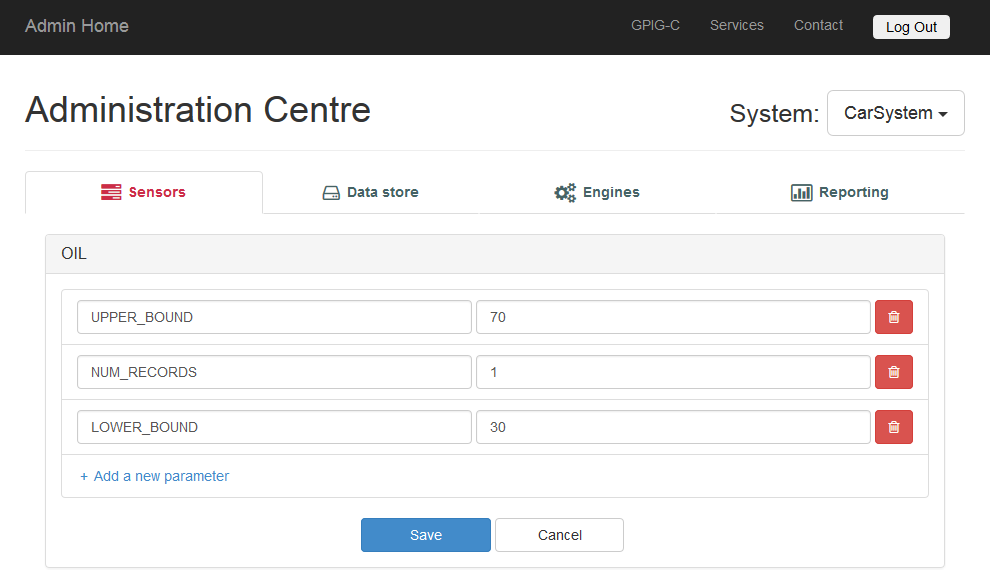
\includegraphics[width=\textwidth]{images/admin-centre_sensors.png}
        \caption{Sensors}
        \label{fig:admin-centre_sensors}
    \end{subfigure}
    ~
    \begin{subfigure}{0.49\textwidth}
        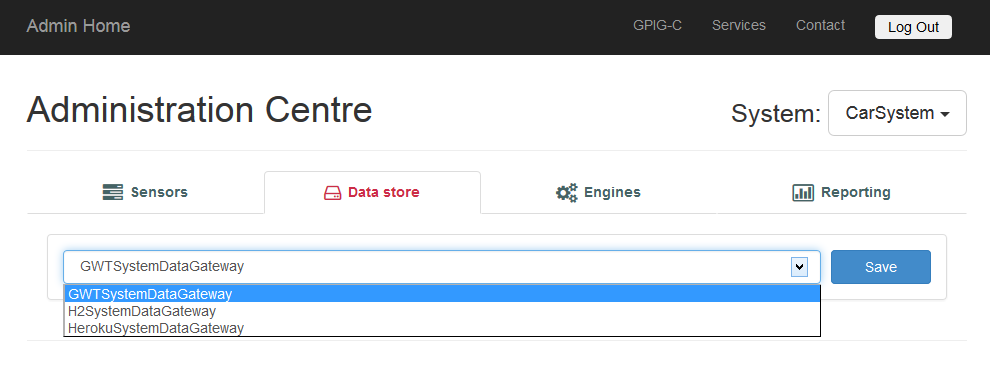
\includegraphics[width=\textwidth]{images/admin-centre_data.png}
        \vspace*{1.18cm}
        \caption{Datastore}
        \label{fig:admin-centre_data}
    \end{subfigure}
	\vspace{0.3cm}

    \begin{subfigure}{0.49\textwidth}
        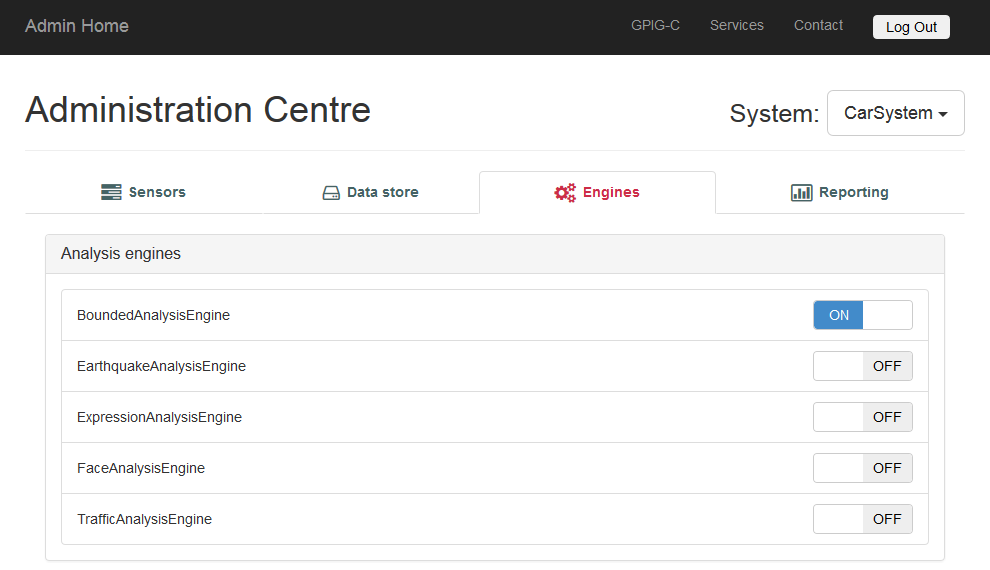
\includegraphics[width=\textwidth]{images/admin-centre_engines.png}
		\vspace*{0.95cm}
        \caption{Engines}
        \label{fig:admin-centre_engines}
    \end{subfigure}
	~
	\begin{subfigure}{0.49\textwidth}
        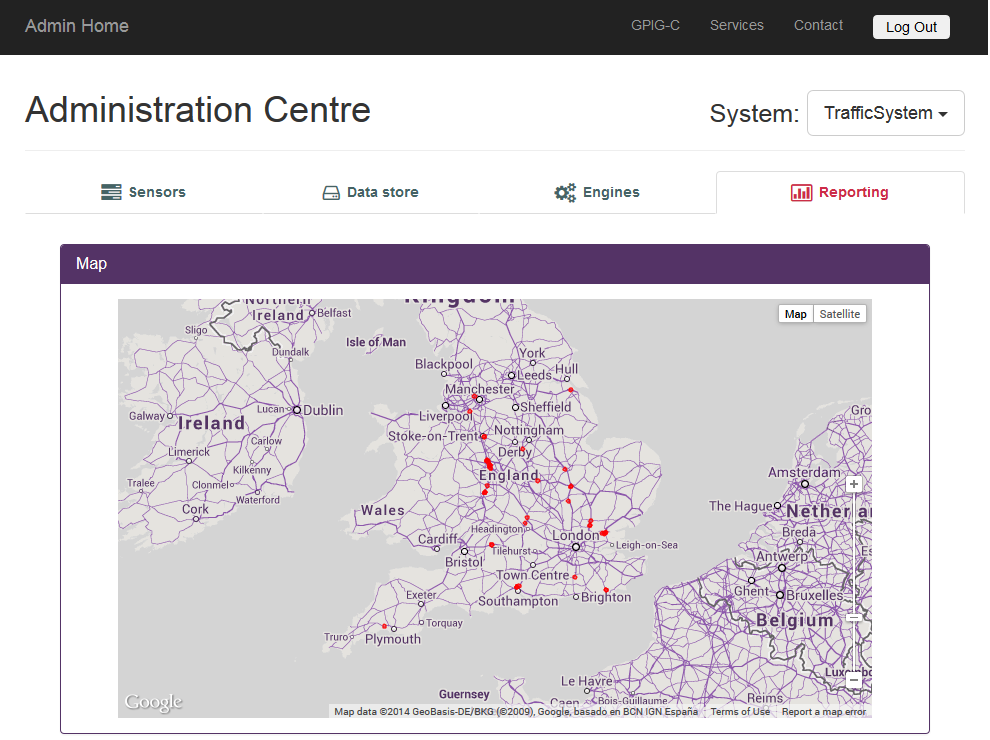
\includegraphics[width=\textwidth]{images/admin-centre_report.png}
        \caption{Reporting}
        \label{fig:admin-centre_report}
    \end{subfigure}
    \caption{Screenshots of the Admin Centre.}
	\label{fig:admin-centre}
\end{figure}

\subsection{Project Building}

The implementation consists of a number of independent software projects which must be built separately and then collated into a final distribution. A number of tools have been used to aid this build process. 

Java applications are typically bundled into Java Archive (JAR) files. By default, libraries that are required by an application must be distributed together with the JAR. This is inconvenient for current distribution because many files must be distributed together. To avoid this, the One-JAR build tool \cite{onejar} is used. It allows an application and its dependencies to be bundled into a single JAR file. In the future, the HUMS may be distributed through system-dependent package managers which handle dependencies automatically.

Apache Ant build scripts \cite{ant} are used to build most of the projects. Much of the build process is common to all projects and so this behaviour has been extracted out into \texttt{tools/common-ant.xml}. This has the following benefits:

\begin{itemize}
\item Projects need only specify build requirements that are project-specific in their respective \texttt{build.xml} files.
\item Projects can be built for different platforms simply by changing a property of the build script.
\item Libraries that are common to multiple projects need not be duplicated between those projects.
\item The build script will perform the bundling of libraries using One-JAR.
\item The entire build process can be performed using a single command.
\end{itemize}

A global \texttt{build.xml} file is provided in the source root directory which builds all projects and combines them into a distributable for the requested platform.

%-------------------------------------------------------------%
%-----------------------TESTING-----------------------%
%-------------------------------------------------------------%
\section{Testing}
\label{sec:testing}
With our design and implementation updated from the Interim Report, we iterated on the test plan created previously, updating it to verify that our updated solution performed as desired and fulfilled the specified requirements.

The test plan has been improved and expanded upon in this iteration to include new components. The \emph{Tracability Matrix} in Table~\ref{tab:traceability} shows the mapping between each requirement and the test classes used to verify it. Not all requirements are included, as they can not all be verified through testing. The testing performed is split into five distinct categories --- acceptance, system, integration, unit, and inspection testing --- as explained in the Interim Report. 

When performing acceptance testing, we communicated with the Customer about proposed functionality and features of our HUMS, and kept them up-to date on what we had achieved. We also expect that the feedback from this report will fold back into our acceptance testing. 

In addition to the tests described in Table~\ref{tab:traceability}, inspection testing also performed when deploying our HUMS across various networked machines, and operating systems, to verify that the HUMS acted as expected. 

Below, the main modules, shown previously in Figure~\ref{fig:modules}, are explained in terms of how testing has allowed us to verify that they fulfil requirements:
\begin{description}
  \item[Core] The HUMS Core includes a \texttt{Shell} providing a GUI and managing execution of the HUMS. This includes listening for changes to engines, thus fulfilling \emph{FR.12} and \emph{FR.4.1.2}, and managing the use of configuration files, helping to fulfil \emph{NFR.14}. Unit tests and manual inspection were used to verify proper operation.

  \item[Data Emitter] The purpose of the Data Emitters is to run continuously, monitoring a Consumer system and passing data the HUMS, thereby fulfilling \emph{FR.1.2}. We completed inspection testing to verify that data was received, along with running the program for several hours to verify that it continued to function correctly.

  \item[Data Input Layer] For the Data Input Layer, it is essential that large amounts of data can be received in parallel. We verified this by inspection testing, and also by running multiple Clients simultaneously and checking that the data from all Clients was correctly recorded, thus verifying \emph{FR.1.1}.

  \item[Data Abstraction Layer] The Data Abstraction Layer's key attributes are availability and performance. The mere existence of the \texttt{SystemDataGateway} interface verifies \emph{FR.3.1}. At the unit testing level, as part of TDD, we verified \emph{FR.3} by testing that data transformation functions used within this layer worked as expected, such as the serialisation of objects using JSON.

  \item[Analysis Controller] Due to the central role played by the \texttt{Analysis Controller}, we identified its key attributes as performance and testability. We utilised Mockito~\cite{mockito} to provide isolated unit tests, confirming that Notifications are only triggered when appropriate, satisfying \emph{FR.7} and \emph{FR.9}. Class loading was used to load analysis engines for the prototype, confirmed to be working via inspection and integration testing, verifying \emph{FR.12}.

  \item[Analysis Engine] For the analysis engines, we created unit tests to verify each aspect of the different engines as per \emph{FR.7} and its refinements. 

  \item[Notification Controller] We created multiple unit tests to verify the functionality of the Notification controller as per \emph{FR.8} and \emph{FR.9}. Mockito was used to isolate the class, allowing for a true unit test. We verified that a Notification is generated when analysis has indicated it should be and that Notifications were only sent once to avoid spamming.

  \item[Notification Engine] The functionality of the example Notification engines is tested using unit testing. The tests use each Notification Engine to send a message to a specified recipient or device, with a given subject and message, then verify that the Notification is successfully sent and received, inspecting it to ensure that the correct information is included. This satisfies \emph{FR.9} and \emph{FR.11}.

  \item[Admin Centre] One of the major features of the Admin Centre is to modify configuration files, thereby fulfilling \emph{FR.4.1.1}. The Admin Centre is web based so testing was primarily performed manually through inspection.

  \item[Reports Engine] Reports Engines are again web based and tested by inspection to ensure the data appeared as desired. This reporting ensured \emph{FR.10} was met.

\end{description}

\tableformat{ p{1.8cm} p{4.7cm} p{1.9cm} X }
{ 	\hline
    Requirement & Test Classes & Type & Details \\
    \hline

    \fr{1.1}   & N/A & Inspection & Use Datastore consoles and viewers to verify data storage \\
    \fr{1.2}   & N/A & Inspection & Verify by observing output in Admin Centre \\
    \fr{2}   & SystemDataTest, \newline EmitterSystemStateTest & Unit & Verify existence of timestamp \\
    \fr{3}    & SystemDataTest, \newline EmitterSystemStateTest, \newline QueryResultTest & Integration, Unit & Verify reading and writing to Datastores, create and parse JSON \\
	\fr{3.1}   & GWTSystemDataGatewayTest, \newline H2SystemDataGatewayTest, \newline HerokuSystemDataGatewayTest & Unit & Verify that different Datastores work correctly and interchangeably \\
	\fr{4.1.1} & N/A & Inspection & Verify configuration files can be changed through the Admin Centre \\
	\fr{4.1.2} & ConfigParserTest & Unit, \newline Inspection & Verify changes to the configuration file are detected and acted upon \\
	\fr{7}     & AnalysisEngineTest, \newline DataEventTest & Unit & Verify events are triggered by analysis where appropriate \\
    \fr{7.1}   & AnalysisControllerTest, \newline NotificationGeneratorTest & Unit,\newline Inspection & Verify notification flag is set and queried to manage Notification frequency \\
    \fr{7.4}   & AnalysisControllerTest & Unit & Verify generation of Events \\
	\fr{8}     & NotificationEngineTest & Unit & Verify the specified Notification cool down period is adhered to \\
    \fr{9}     & EmailNotificationTest, \newline SMSNotificationTest, \newline TwitterNotificationTest & Unit, \newline Inspection & Verify the sending of Notifications \\
	\fr{10}    & N/A & Inspection & Verify appropriate graph and map reports can be generated with correct data \\
	\fr{12}    & N/A & Inspection & Verify that the Core detects and loads new engines \\
    \nfr{6}    & N/A & Inspection & Verify existence of all test levels \\
	\nfr{14}   & ConfigParserTest, \newline ParameterTest, \newline ClientSensorTest, \newline ClientSystemTest & Unit, \newline Inspection & Verify that configuration files are understandable and parseable \\
}
{The traceability table showing the mapping between requirements and existing tests.}{tab:traceability}


%-------------------------------------------------------------%
%-----------------------PROTOTYPE-----------------------%
%-------------------------------------------------------------%
\section{Prototype Evaluation}
\label{sec:prototype}

In this section, our prototype implementation is evaluated to assess how well it has met our specified requirements and quality attributes. This includes evaluating how it performs with the two test applications provided by the Customer, and helps to assess the overall implementation work that has been completed.

% an evaluation involving at least two distinct applications, with special attention to the "tailorability" of the solution for different applications, and including results for the test applications supplied by The Customer; (Include instructions for replicating such results.)

%  How thoroughly has it been evaluated, how diverse are the applications that have been tested, and how good are the results?

\subsection{Evaluation Against Requirements, Quality Attributes, and Scenarios}
\label{sec:req_eval}

In order to properly evaluate our solution, we must consider its limitations and strengths. Previously, Section~\ref{sec:testing} discussed how our test plan allowed us to verify a number of our requirements. In this section we consider whether we have met the requirements which were not verified through testing, how we have maximised the utility of our key quality attributes, and whether our HUMS responds as expected in the scenarios detailed in Section~\ref{sec:scenarios}.

Table~\ref{tab:functionalEval} shows which functional requirements we were able to meet with our prototype, describing how we checked these requirements were met if verification was not completed through testing, as previously detailed. Where requirements have not been met, an explanation has been given as to why this was the case, and how in the future they would be achieved. Table~\ref{tab:nonfunctionalEval} details the same information for the non-functional requirements.

These tables show how our implementation has met the majority of our requirements, however is limited in terms of security and with the services offered through our SaaS deployment. We chose not to fulfil these requirements as part of the prototype as we did not feel that they would be as important to the Customer, at this stage, than more basic functionality.

\tableformat{ p{2cm}  p{2cm} X }{
Requirement & Verified? & Reasoning \\ \hline
\fr{1} & Yes & Inspection testing showed this requirement to be satisfied.\\
\fr{2} & Yes & Unit testing showed this requirement to be satisfied.\\
\fr{3} & Yes & Integration and unit testing showed this requirement to be satisfied.\\
\fr{4} & Partially & Some of the refinements of this requirement were verified through testing, and a snapshot of the configuration file format used is shown in Figure~\ref{fig:configFiles}. Other refinements, concerning storage limits, could not be verified for reasons explained below. \\
\fr{5} & No & Due to timing constraints, we chose not to implement storage quotas for our SaaS distribution of the HUMS as part of this prototype. In the future this requirement would be verified by defining a storage limit through the Admin Centre and attempting to store more data than allowed. It would then be confirmed that a notification is sent and received.\\
\fr{6} & No & For the reasons above, this requirement could not be fulfilled as part of this project. Verification in the future would be similar to \emph{FR.5}.\\
\fr{7} & Yes & Unit and inspection testing showed some refinements of this requirement to be satisfied. Others are verified through the mere existence of functioning engines which implement the \texttt{AnalysisEngine} interface.\\
\fr{8} & Yes & Unit testing verified that cool down periods function correctly in our implementation. \\
\fr{9} & Yes & Unit and inspection testing verified that all implemented Notification engines correctly send Notifications.\\
\fr{10}& Yes & Unit testing, and the existence of our web based reporting tools, verified this requirement.\\
\fr{11}& Yes & The phone system, created as part of the Android application, proves that our HUMS is capable of changing the behaviour of the Consumer system it is monitoring.\\
\fr{12}& Partially & Dynamic class loading is fully functional, and verified through testing. However, we have not implemented a secure user system as part of this prototype due to time constraints, meaning any user with write-access could add or remove engine files. \\
}{Verification of functional requirements.}{tab:functionalEval}


\tableformat{ p{2cm}  p{2cm} X }{
Requirement & Verified? & Reasoning \\ \hline
\nfr{1} & Partially & Remote Datastores have been tested, and data can continue to be accessed after local hardware modifications. Local Datastores persist as desired through some hardware modifications, but more thorough testing is required.\\
\nfr{2} & Yes & A \emph{User Manual} has been provided with our prototype implementation. \\
\nfr{3} & Yes & Our HUMS can be utilised regardless of geographic location, as the main monitoring site is accessible from the web. Furthermore, the Data Emitters can be run separately from the main System, for example, on an embedded system. \\
\nfr{4} & No & Though security is a key quality attribute of our System, and has been considered throughout development, we have not actually implemented any security standards due to time constraints. We have however ensured that the protocols used can be secured in the future.\\
\nfr{5} & No & As above.\\
\nfr{6} & Yes & Section~\ref{sec:testing} explains how our System was tested, and this section explains which requirements have been met.\\
\nfr{7} & Partially & The Customer has accepted our previous implementation and provided feedback on our decisions throughout this phase. Acceptance of this final prototype will fulfil this requirement.\\
\nfr{8} & Yes & Our included \texttt{EmitterLauncher} had been integration tested with the System, and can concurrently run five Data Emitters and dispatch Notifications to five Output Clients.\\
\nfr{9} & Yes & All Datastores currently used with our HUMS have an uptime which satisfies this requirement.\\
\nfr{10} & Yes & Redundant copies of data are created when using the remote Datastores and backups can easily be manually created for the local Datastores. \\
\nfr{11} & Yes & Timestamps are stored with the data, and have been verified to be within $5$~ms of UTC. \\
\nfr{12} & Yes & The timings have been checked for all implemented notification engines, and are less than $5$~ms. \\
\nfr{13} & Yes & Data has been sent to the HUMS in a variety of popular formats, including JSON, XML, and key-values, and then correctly stored.\\
\nfr{14} & Yes & The configuration file has been stored in JSON, and is shown in Figure~\ref{fig:configFiles} to be human readable.\\
}{Verification of non-functional requirements.}{tab:nonfunctionalEval}

Having evaluated our solution against the requirements, we must also consider our quality attribute scenarios, designed to test the System's ability to provide the desired responses in interesting contexts. Table~\ref{tab:qasEval} shows the expected responses of our included quality attribute scenarios, and the actual responses of the prototype. For the most part, these responses are as expected. However, not implementing Client authentication in the prototype has led to \emph{QAS.3} not being satisfied, and not having an Admin Centre with fully functional user accounts means that \emph{QAS.4} cannot be entirely fulfilled.


\tableformat{ p{2cm} X X }{
Scenario & Desired Response & Actual Response \\
\qas{1} & The Consumer can modify their configuration file without reinstalling or recompiling the HUMS. & As expected.\\
\qas{2} & A new engine is implemented, tested, and added to the HUMS without loss of service, and without affecting other systems. & As expected, time taken to achieve this was between $2$ and $12$~hours, depending on the complexity of the engines. \\
\qas{3} & An unknown external Client is either authenticated and allowed to access HUMS services, or denied access. & Currently Clients are not authenticated, however, the HUMS only listens for data from systems sending a correct System ID, as declared in the configuration file. \\
\qas{4} & A notification is sent to the Consumer when the HUMS cannot connect to their external Datastore, and the HUMS attempts to reconnect the next time data is received. & A notification is not currently sent to the Consumer, however, the HUMS does attempt to reconnect the next time data is received.\\
}{The desired quality attribute scenario responses and the actual responses of the System}{tab:qasEval}

Throughout the document we have considered our important quality attributes, and referenced features we have implemented in an attempt to increase their utility.

The quality attributes laid out in Section~\ref{sec:scenarios} have been largely satisfied. We feel our emphasis on making our HUMS configurable, flexible, and modifiable has led to it being incredibly tailorable. This has been proven with the number of different applications we have been able to monitor, and how easily we have integrated them.

In addition to this, we performed a small UX study within the department to help us ensure that our HUMS Core interface and Admin Centre were easy to use. Results of the study led us to change the font of our consoles to an easier to read monospace font, and to add a `clear console' button, allowing old information to be deleted, making updates easier to see. We also found that users wanted to be able to toggle engines on and off using the Admin Centre, rather than manually selecting which ones they would like to use. We acted upon this feedback and changed our interfaces appropriately.

\subsection{Evaluation on the Customer's Test Applications}
\label{sec:test_app1}

We decided to monitor the memory and CPU usage of the first test application, using SIGAR to monitor CPU usage and JMX to monitor memory. JMX was used as the JVM has a fixed heap sized meaning SIGAR cannot determine what is being used by the application. 

Use of the SIGAR library proved useful when attempting to monitor the second test application, as we were able to reuse much of work. For this test application we also considered monitoring IO operations and network activity. To test whether monitoring these would be a good use of our time we used \emph{iotop}~\cite{iotop} to examine the application's IO operations and found nothing notable, then also used \emph{Wireshark}~\cite{wireshark} to examine network activity but found none. 

With this in mind, we decided to monitor the process memory usage, CPU usage, state (idle, running, sleeping, stopped, or zombie), working directory, number of threads, and which processor it was last run on, allowing us to reuse the SIGAR library. SIGAR is also capable of monitoring networking and file system metrics, however, we did not feel that this was useful information when considering the second test application.

\subsection{Evaluation of the HUMS SaaS}
\label{sec:hums_saas}

In the Interim Report we proposed an innovative deployment option for our HUMS as a System as a Service (SaaS) solution, allowing multiple Consumers to use the same central HUMS. This removes the complexity of setting up and managing the System themselves, whilst being configurable through the use of custom engines and configuration files.

This deployment is possible as components of our HUMS can run from different locations. With our HUMS implementation the SaaS solution can be achieved by running multiple Cores on the same server, with one Core for each Consumer. This is not ideal, as a new Core instance for a new Consumer would have to manually be started, but does successfully enable this type of deployment.

Ideally, only a single instance of the Core would be needed and would be able to handle multiple Consumers' configurations. This is a future possibility for the System as only small parts of the Core would need to be modified and all other components, including engines, could remain the same.

\subsection{Evaluation of Additional Engines}
\label{sec:additional}

Providing support for multiple kinds of data store technologies within the HUMS prototype proved to be a relatively straightforward process. As part of our prototype, we added both local and remote SQL, NoSQL and distributed Datastores, showing our architecture yields a high level of both interoperability and flexibility. The fact that we can switch between these by changing a configuration file at runtime, without any code being written, shows a high level of configurability and usability, since consumers with even low levels of technical knowledge can implement these changes.

The \texttt{FaceAnalysisEngine} provided an example of a complex, domain-specific, analysis engine being easily built on top of the generic interface. The configuration file allowed easy description of the faces to be accepted by storing a relative path to a face description file, and the Java interface provided a simple mechanism for retrieving data from the Sensors. This engine showed that even highly tailored engines comfortably fit within our plugin model, giving strong evidence that our prototype is highly tailorable and can be used across domains.


%-------------------------------------------------------------%
%---------------------COMMUNICATION-------------------%
%-------------------------------------------------------------%
\section{Customer Communication}
\label{sec:customer_comms}

We maintained communication with the Customer throughout the phase of this report, with emails exchanged every few weeks. The first feedback received from the Customer came from the Interim Report, and a face-to-face meeting with the Customer. The Customer give us a number of areas to work on for this report, including better explaining how we considered risks, how we can improve the presented views of our System architecture, and explicitly stating our quality attribute scenarios. This feedback has been clearly acted upon in this report.

During email communication with the Customer, we attempted to resolve an issue they had accessing the web sources that were produced as part of the Interim Report. Once this had been resolved, the ideas behind the configurable engines architecture was agreed to be a good strategy. We then asked about which qualities the customer would like us to focus on during development, suggesting that flexibility and interoperability appear important. The Customer replied highlighting that configurability is also key quality and should be considered, and this led to the creation of the configuration file system. 

Further information about how development was progressing and proposals for future work was exchanged, ensuring the Customer was kept up-to-date and that the project remained on the right track. This included information about how the system would meet the previously highlighted configurability quality, and how this could be achieved at both compile time and runtime. Discussion about Datastores was also useful and revealed the possibility of adding distributed Datastores to our implementation. This feedback was taken on board leading us to add \emph{Neo4j} and \emph{TempoDB} to our implementation.


%-------------------------------------------------------------%
%----------------------CONCLUSION----------------------%
%-------------------------------------------------------------%

\section{Conclusion}
\label{sec:conclusion}

This report has presented the updated design and implementation of our HUMS solution, highlighting any progress since the Interim Report. It focusses particularly on the technical development undertaken and evaluates the implemented System against the identified requirements.

Whilst we were not able to implement a complete solution within the constraints of the project, and not all functional requirements have been met, the prototype solution is a promising start towards a complete system. Whilst developing the prototype and the example applications, we have shown that it supports many of the key quality attributes. For example, we have demonstrated the ease with which the System can be extended by implementing new engines.

In this way, we have focussed mostly on the quality attributes that pertain to the functionality required by a HUMS---that is, sensing, storing, analysing, and reporting---and less on those quality attributes required for a real-world application (such as security). Doing so has allowed us to demonstrate the user-facing behaviour and feasibility of the HUMS, while later development can tackle the details of Consumer deployment.

\subsection{Reflection}
\label{sec:reflection}

In hindsight, to improve our final product and streamline our process, a number of development tasks could have been performed differently.

A more thorough evaluation of early prototypes should have been performed to ensure that all components were working according to the functional requirements. For example, it was discovered late in development that the functionality for dynamically loading engine class files only checked if those files existed and then simply instantiated the engines that were compiled into the Core. This violated requirement \emph{FR.12}, and wasted development time. Such problems could have been avoided if they had been identified earlier by more thorough testing or better team communication.

Software engineering design patterns were not explicitly identified during the interim development, meaning that much of the software architecture needed to be heavily modified in this phase as the ramifications of the changes to our design decisions became clear.

The development plan in the previous report did not fully account for external pressures, such as other modules. This was previously identified as risk \emph{R.2}. Had this been appropriately accounted for, the available time could have been used more effectively and we could have avoided running into our contingency time.

The necessary build tools could have been determined and configured at an earlier stage, allowing later work to focus more on development of the HUMS itself rather than solving build issues. This would also have allowed the use of continuous integration for greater quality control and hence a more efficient development process.

Our use of the SWT library for building the user interface cost a surprising amount of time as appropriate native libraries had to be bundled for each platform, complicating the build process. Whilst we were pleased with the final result, this may not have been worth the time spent on it.

The implementation of the graph database, \emph{Neo4j}, provided numerous challenges and therefore proved time consuming. Team members were most familiar with modelling relational and key-value data, making the experience quite jarring. In hindsight, more time should have been devoted to the implementation of unfamiliar datastore technologies.

\clearpage

\bibliography{report-refs}
\bibliographystyle{IEEEtran}
\end{document}
